\documentclass[
    draft=true,
    paper=a4,
    fontsize=11pt,
    twoside=true,
    captions=tableheading,
    british, ngerman,
]{scrreprt}
\usepackage[headsepline]{scrlayer-scrpage}
\pagestyle{scrheadings}
\automark[section]{chapter}

\usepackage{babel}

\usepackage{lipsum}

\usepackage[utf8]{inputenc}
\usepackage[T1]{fontenc}
\usepackage{microtype}

\usepackage{newpxtext}
\usepackage{newpxmath}

%\usepackage{float}
\usepackage{booktabs}
\usepackage{amsmath, amssymb}
\usepackage{csquotes}
\usepackage{graphicx}
\usepackage[labelformat=simple]{subcaption}
\renewcommand\thesubfigure{(\alph{subfigure})}

\usepackage{siunitx}
\sisetup{locale = DE}

\usepackage[
    colorlinks=true,
    allcolors=black,
    urlcolor=blue,
]{hyperref}

\setkomafont{captionlabel}{%
    \bfseries
}
\setkomafont{caption}{%
    \bfseries
}
\setcapindent{0em}

\usepackage{listings}
\usepackage{xcolor}

\definecolor{dark-grey}{rgb}{0.3, 0.3, 0.3}
\definecolor{comment-green}{rgb}{0.0, 0.6, 0.0}

\lstset {
    aboveskip = 1em,
    belowskip = 1em,
%    abovecaptionskip=1em,
    belowcaptionskip=1em,
%    backgroundcolor = \color{black!5},
    basicstyle = \ttfamily,
    caption = \lstname,
    commentstyle = \itshape\color{comment-green},
%     frame = single,
    rulecolor = \color{black!10},
    keywordstyle = \color{blue},
    numbers = left,
    numbersep = 12pt,
    numberstyle = \footnotesize\ttfamily\color{dark-grey},
    stepnumber = 1,
    showstringspaces = false,
    tabsize = 4
}

\usepackage[
    backend = biber, % Sets biber as backend.
    style = authoryear-icomp, % Use [author, year] citing with ibid. when duplicate.
    maxcitenames = 2, % Truncate lists above 2 entries (e.g. names) when citing.
    mincitenames = 1, % Truncate to 1 entry (e.g. names) when citing.
    maxbibnames = 3, % Truncate lists above 3 entries (e.g. names) in bib.
    minbibnames = 3, % Truncate to 3 entries (e.g. names) in bib.
    backref = true, % Show reference to page.
    backrefstyle = three, % Will compress sequences of three pages or mmore, e.g. 1,2,3,5,7 to 1-3,5,7.
    isbn=false,
    url=false, % Note: @Online references will stay unaffected (yay).
    giveninits=true, % Show only initials for given names.
    uniquename=init, % To disable conflict warning because of giveninits.
]{biblatex}
% Space out bib entries a bit.
\setlength\bibitemsep{1.5\itemsep}
% Put lastname before firstname.
\DeclareNameAlias{sortname}{family-given}
% Separates author names with semicolon instead of comma.
\renewcommand{\multinamedelim}{\addsemicolon\space}

% Bib resources.
\addbibresource{../references/references.bib}
\addbibresource{../references/websites.bib}
\addbibresource{../references/unpublished.bib}

\newcommand{\quelle}[1]{{\normalsize \emph{(Quelle: #1)}}}

\newcommand{\quelle}[1]{%
    \mbox{\itshape(Quelle:\ #1)}
}
\newcommand{\wifi}{\mbox{Wi-Fi}}
\newcommand{\unity}[1]{#1}
\newcommand{\imagebox}[1]{%
	{\color{black!25}%
	\framebox[\textwidth]{\normalcolor #1}}%
}


%\includeonly{titlepage, declaration_of_originality, thanks, abstract}

\begin{document}

\pagenumbering{roman}
\begin{titlepage}
	\begin{center}
		\LARGE\textbf{\textsc{Universität Bremen}}\\
		\large\textbf{\textsc{Fachbereich 3: Mathematik/Informatik}}\\
		\vspace{2cm}
		\LARGE \textbf{\textsf{Arbeitstitel}} \\
		\vspace{2cm}
		\LARGE\textbf{\textsc{Masterarbeit}}\\
		\vspace{0.5cm}
		\large
		im Studiengang\\
		\enquote{Informatik Master of Science}\\
		\vspace{1cm}
		\normalsize
		vorgelegt am: \dots \\
		\vspace{3.5cm}
	\end{center}
	\vfill
	\hrule
	\vspace{1em}
	\normalsize{
		\begin{tabular}{ll}
			Name: & {Ralf Manuel Morawe} \\
			Matrikelnummer: & {2615732} \\
			Studiengang: & Informatik\\
			Fachsemester: & 4\\
			Erstgutachter: & {Prof. Dr. Johannes Schöning} \\
			Zweitgutachter: & {\dots} \\
		\end{tabular}\\
	}
\end{titlepage}
\cleardoublepage
\chapter*{Selbstständigkeitserklärung}
\thispagestyle{empty}

Hiermit erkläre ich, dass ich die vorliegende Arbeit selbstständig angefertigt, nicht anderweitig zu Prüfungszwecken vorgelegt und keine anderen als die angegebenen Hilfsmittel verwendet habe. Sämtliche wissentlich verwendete Textausschnitte, Zitate oder Inhalte anderer Verfasser wurden ausdrücklich als solche gekennzeichnet.\\[2ex]
Bremen, den \today\\[6ex]

\begin{tabular}{l}\toprule
	\centering\footnotesize Ralf~Manuel~Morawe
\end{tabular}
\cleardoublepage
%\chapter*{Danksagung}
\thispagestyle{empty}
\lipsum[10-11]
\cleardoublepage
%\chapter*{\abstractname}
\thispagestyle{empty}
\lipsum[1]

\cleardoublepage

\begin{otherlanguage}{british}
\chapter*{\abstractname}
\thispagestyle{empty}

\lipsum[2]

\end{otherlanguage}
\cleardoublepage

\tableofcontents
\cleardoublepage
\pagenumbering{arabic}

%\chapter{Einleitung}
\label{chap:einleitung}

Durch den technischen Fortschritt in den letzten Jahren hat sich der Einsatz von \emph{Augmented Reality} (AR) und \emph{Virtual Reality} (VR) in verschiedenen Anwendungsbereichen etabliert \parencite{Krevelen2010, Zhao2009, Sharples2008, Jung2008}.
Als Nutzerschnittstelle dienen dienen in vielen Anwendungen Smartphones, da die Sensoren (Kameras, Gyrosensor etc.) nun ausreichen, um einfache AR-/VR-Inhalte zu präsentieren \parencite{Li2017b,Feng2017,Yoo2015,Mulloni2012}.
Neben Smartphones ermöglichen Head-Mounted Displays (HMDs) die Anzeige von \emph{Mixed-Reality-} (MR) und VR-Inhalten.
Beispielsweise sind hier die \emph{Microsoft HoloLens} \parencite{Microsoft2018} als AR-HMD oder die \emph{Oculus Rift} \parencite{Facebook2018} und \emph{HTC Vive} \parencite{HTCCorporation2018} als VR-HMD zu nennen (siehe \autoref{fig:devices}).
\begin{figure}[hb]
    \centering
    %\imagebox{%
    \begin{minipage}{0.3\textwidth}
        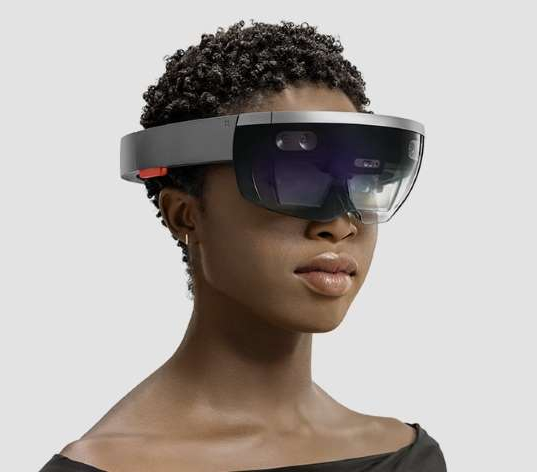
\includegraphics[width=.9\linewidth]{figures/Microsoft2018_HoloLens_worn}
    \end{minipage}%
    \hfill
    \begin{minipage}{0.45\textwidth}
        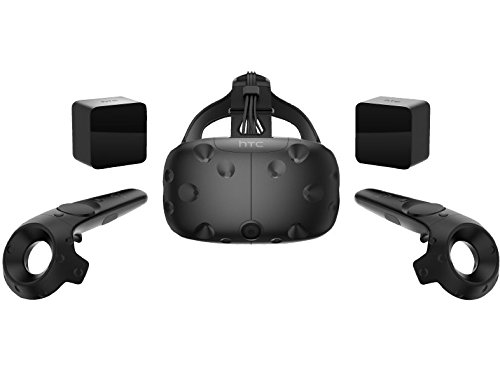
\includegraphics[width=.9\linewidth]{figures/htc_vive}
    \end{minipage}%
    \hfill
    \begin{minipage}{0.25\textwidth}
        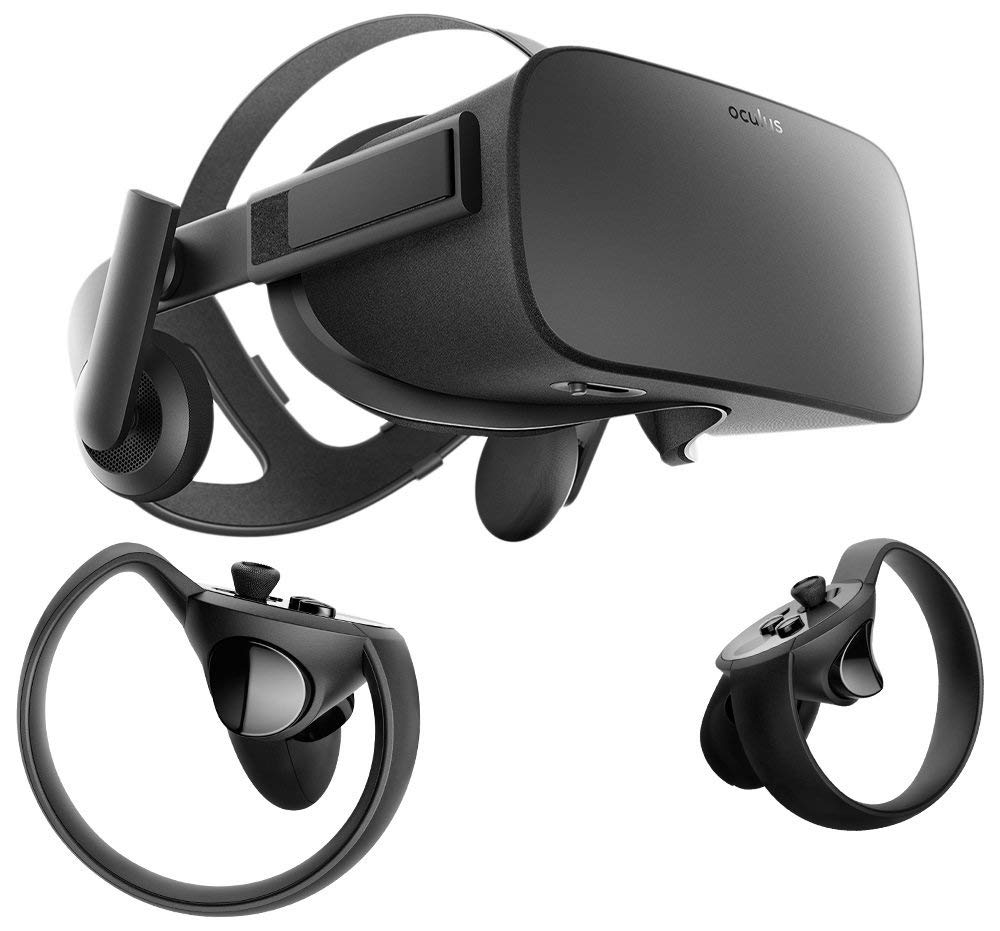
\includegraphics[width=.9\linewidth]{figures/oculus_rift}
    \end{minipage}%
    %}
    \caption{Diverse MR- und VR-HMDs. Microsoft HoloLens (Links), HTC Vive (Mitte) und Oculus Rift (Rechts). \quelle{\cite{Microsoft2018, Amazon2018b, Amazon2018}}}
    \label{fig:devices}
\end{figure}

Bei AR wird die Grenze zwischen dem Reellen und dem Virtuellen aufgehoben, indem virtuelle Inhalte in Echtzeit mit sechs Freiheitsgraden in die reale Welt überlagert werden.
\autoref{fig:mrtouch} zeigt z.B., wie virtuelle Nutzungsschnittstellen in die physische Welt platziert werden und über Berührungsinteraktion gesteuert werden können.
In der Vergangenheit wurde von Forschern AR unter anderem eingesetzt, um räumliche Informationen in der Umgebung von Nutzern anzuzeigen.
Beispielsweise wird die Navigation zwischen zwei Punkten augmentiert.
Die bisherigen Ansätze fokussieren die AR-unterstützte Schritt-für-Schritt-Navigation \parencite{Hoellerer1999, Hashish2017, Mulloni2012} und die Augmentierung von realem Kartenmaterial \parencite{Rohs2009, Morrison2009, Reitmayr2005}.
\begin{figure}[ht]
    \centering
    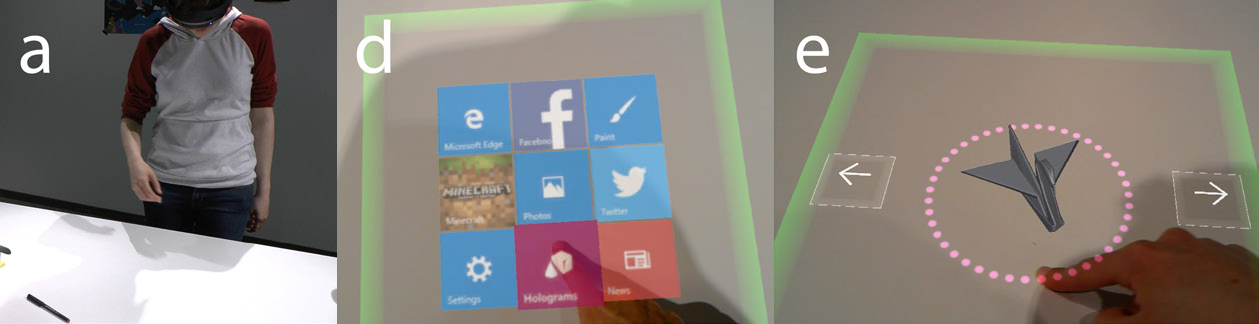
\includegraphics[width=\textwidth]{figures/mrtouch}
    \caption{Virtuelle Interfaces werden auf physischen Oberflächen platziert und mittels Berührungsgesten aktiviert. \quelle{\cite{Xiao2018}}}
    \label{fig:mrtouch}
\end{figure}

\section{Motivation und Ziel der Arbeit}
\label{sec:motivation_ziel}
Das Ziel \emph{dieser} Arbeit ist die Entwicklung einer neuartigen Form, räumliche Informationen mithilfe eines HMDs in eine AR-Szene zu integrieren: die \textbf{Megamap}.
Als Megamap wird in dieser Arbeit einer Kartendarstellung definiert, bei der ein dreidimensionales Abbild der Umgebung um den Nutzer herum gezeigt wird.
Die Karte ist in einem verkleinerten Maßstab zur Umgebung und ist in diese verankert.
Das bedeutet, wenn sich der Nutzer in der Welt bewegt, dann bewegt er sich auch auf der Karte.
Die virtuelle Karte verhält sich somit, als sei sie ein reales Objekt in der Umgebung.

Die ursprüngliche Idee für die Megamap-Darstellung stammt aus dem Spiel \emph{Tom Clancy's The Division} (TCTD) \parencite{Ubisoft2018} (siehe \autoref{fig:megamap}).
Eine Karte der Umgebung (eine Variante von New York) wird mit relevanten Spielobjekten und Ortsnamen \emph{im Spiel} als AR-Interface um den Charakter herum angezeigt.
Die Karte erlaubt dem Spieler unter anderem, Wegpunkte festzulegen (Navigation), interessante Punkte in der Umgebung anzuzeigen und zu filtern (Exploration) sowie die Ansicht durch Verschieben und Zoomen der Karte anzupassen.
Ebenso werden Missionsziele, andere Charaktere und Events durch Icons in der Karte hervorgehoben.
All diese Informationen sind vom aktuellen Kontext des Spiels abhängig.
Das heißt, es werden nur Informationen angezeigt die für die aktuelle Spielsituation des Spielers relevant sind.
\begin{figure}[t]
    \centering
    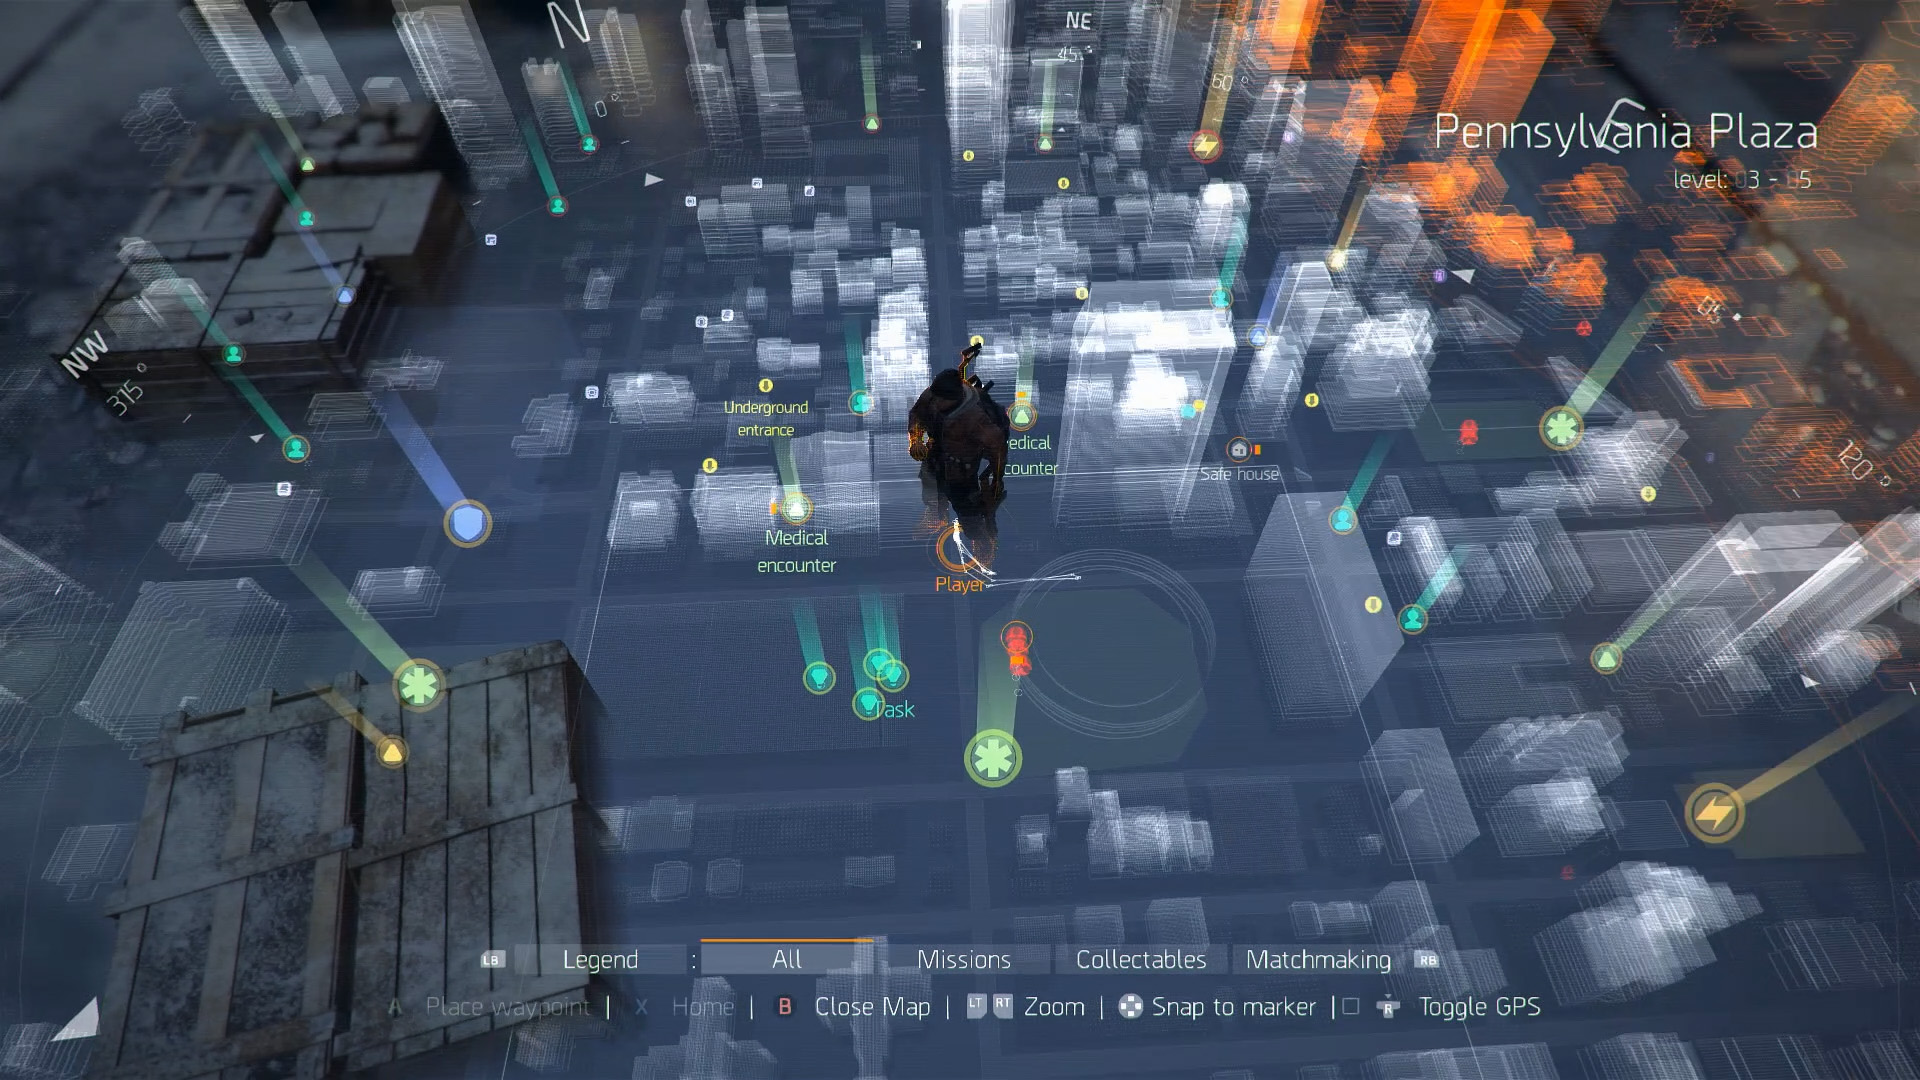
\includegraphics[width=\textwidth]{figures/the_division_megamap.jpg}
    \caption{Die \enquote{Megamap} aus \emph{Tom Clancy's The Division}. Symbole zeigen Missionsziele, Gegenstände und wichtige Orte im Spiel. \quelle{\cite{MYDIVISION.NET2014}}}
    \label{fig:megamap}
\end{figure}

%Eine Kartendarstellung existiert in dieser Form bisher nur im Spiel.
%In der realen Welt werden Karten zwar zunehmend durch AR/VR unterstützt.
%Eine Anwendung wie die Megamap aus TCTD, bei der die Karte in die Umgebung integriert ist, gibt es bisher aber noch nicht.
%Dafür gibt es mehrere Gründe:
%\begin{enumerate}
%    \item Die bisherigen Lösungen zur AR-unterstützten Kartenexploration stützen sich meistens auf die Überlagerung von virtuellen Information auf physische Objekte, beispielsweise eine reale Karte.
%    Dabei wird häufig ein Smartphone als \emph{Magic Lens} (\enquote{Magische Lupe},~\cite{Bier1994}) eingesetzt, auf dem die virtuellen Informationen vor dem Hintergrund der Kamera angezeigt werden.
%    Solch ein Ansatz ist jedoch nur Bedingt für den mobilen Einsatz geeignet.
%    Einem Fußgänger würde das gleichzeitige Halten einer Karte und eines Smartphones schwerfallen, besonders während des Laufens.
%    Auch der Einsatz eines Projektors, der die Informationen auf eine Karte projiziert, ist hierfür nicht geeignet.
%
%    \item Die durch virtuelle Helfer unterstützte Navigation ist ein Ansatz, der sich in der Forschung häufig finden lässt.
%    Allerdings ist die reine Navigation nicht der einzige Anwendungsfall in Bezug auf Kartenanwendungen.
%    Wie \textcite{Reichenbacher2001} detailliert beschreibt gibt es weitere Anwendungsfälle, die sich unter dem Oberbegriff der \emph{Kartenexploration} zusammenfassen lassen.
%    Darin eingeschlossen sind zum Beispiel die zuvor erwähnten Szenarios der Restaurantsuche oder der Anzeige von Fahrt- oder Öffnungszeiten.
%    Allgemein gesagt geht es bei der Kartenexploration um die \enquote{Entdeckung} von Orten anhand von Karten.
%    Diese Anwendungsfälle werden jedoch, in Bezug auf Unterstützung durch AR/VR, seltener behandelt als die Unterstützung der reinen Navigation.
%
%    \item Die Ansätze in der Literatur nutzen in der Regel Smartphones oder andere Handgeräte.
%    Obwohl die Entwicklung dieser Geräte technologisch rasch voranschreitet, sind sie auf die Möglichkeiten der Kamera-Bildsensoren, Gyrosensoren und GPS-Sensoren beschränkt.
%    Z.B. ist die dreidimensionale Rekonstruktion einer Szene, wenn überhaupt, nur sehr vereinfacht möglich.
%\end{enumerate}
%
%Die Integration der Karte in die Umgebung wäre jedoch von Vorteil.
%Denn eine von der Umgebung getrennte virtuelle Karte, wie es bei vielen aktuellen Smartphone-Anwendungen der Fall ist, kann die Aufmerksamkeit des Nutzers von der eigentlichen Umgebung ablenken.
%Die Nutzer müssen ständig das virtuelle Bild mit ihrer Umgebung abgleichen.
%Dies ist nicht nur ein zusätzlicher mentaler Aufwand.
%Im schlimmsten Fall kann es zu schweren Unfällen kommen wenn die Nutzer auf die virtuelle Darstellung achten oder die dargestellten Informationen beim Abgleich mit der Umgebung fehlinterpretieren \parencites{Medenica2011}{Lin2017}.
%
%Weitere Schwierigkeiten ergeben sich bei der Darstellung von \emph{Indoor}-Karten (Karten von Gebäuden).
%Die Überlagerung von mehreren Stockwerken stellt ebenso ein Problem dar wie die Tatsache, dass das GPS innerhalb von Gebäuden nicht verfügbar ist.
%Daher setzen sich viele existierende Ansätze mit der Navigation oder Lokalisierung innerhalb von Gebäuden auseinander.
%Der Anwendungsfall der Karten\emph{exploration} von Gebäuden wird hingegen bisher wenig behandelt.
%Weil kaum öffentliche Gebäudedaten verfügbar sind (im Gegensatz zu \emph{Outdoor}-Daten wie z.B. von \emph{Open Street Map} \parencite{OpenStreetMapFoundation2018}) wird die Situation weiter erschwert.

Eine Darstellung von räumlichen Informationen als Megamap bietet gegenüber herkömmlichen Ansätzen einige Vorteile:
\begin{itemize}
    \item Durch die Verwendung des HMDs bleiben die Hände der Nutzer frei. %
    Sie können die Karte nutzen und gleichzeitig mit beiden Händen mit der Umgebung interagieren.

    \item Da die Kartenansicht in die Umgebung der Nutzer integriert ist, müssen Nutzer die Kartendarstellung mit der Umgebung nicht wiederholt abgleichen. %
    So wird der Umgebung genug Aufmerksamkeit geschenkt und der mentale Aufwand der Nutzung wird verringert \parencite{Bark2014, Narzt2006, Kim2009}.

    \item Dadurch, dass die Karte in die Umgebung verankert ist und sich mit ihr mitbewegt, kann die Megamap auch während der Fortbewegung genutzt werden.

    \item Mit der Megamap können sowohl Außen- als auch Innenbereiche (z.B. Gebäude) dargestellt werden.
\end{itemize}

Die Recherche des Verfassers ergab keine Anwendungen, die das zuvor beschriebene Konzept einer Megamap umsetzen.
Daher wird im Rahmen dieser Arbeit eine Megamap-Anwendung entwickelt.
Spezifisch zielt die Anwendung auf die Nutzung in Innenbereichen wie Gebäude ab, da bisherige MR-HMDs Probleme mit der Verwendung im Freien aufweisen \parencite{Schroeder2017, Strange2018}.

Da sich außerdem die bisherigen Ansätze mit der Karten\emph{navigation} (\enquote{von A nach B}) beschäftigen, wird in dieser Masterarbeit der Anwendungsfall der Karten\emph{exploration} fokussiert.
Bei der Kartenexploration geht es um die Erkundung von Umgebungen anhand von kontextbasierten Ortsdaten.
Kontextbasierte Ortsdaten sind Daten, die von der aktuellen Situation abhängig sind, wie z.B. der aktuellen Position des Nutzers (\textquote{Wo ist das von mir aus nächste Restaurant?}/\textquote{Wieviele Spielplätze sind in meiner Nähe?}).
Ortsdaten können ebenso von der Zeit abhängen (\textquote{Welche Supermärkte in der Gegend sind geöffnet?}).
Übertragen auf die Innenbereichsnutzung stehen mit der Megamap verschiedene explorative Funktionen bereit, beispielsweise das Suchen nach den Büros von Personen oder den Standorten von öffentlichen Druckern.
Nutzer können sich mit der Megamap einen detaillierten Überblick über das Gebäude verschaffen, in dem sie sich befinden.

Als Zielplattform dient das Vive-HMD.
HMDs haben gegenüber Smartphones einige technische Vorteile.
Positionen und Orientierungen der Nutzer sind über Tracking präziser möglich.
MR-HMDs wie die HoloLens oder die \emph{Magic Leap One} \parencite[siehe \autoref{fig:magic_leap}]{MagicLeap2018} verwenden Infrarotkameras, um Strukturen der Umgebung virtuell in Echzeit zu rekonstruieren.
Die reale Umgebung bleibt dank des durchsichtigen Glases weiterhin sichtbar.
Zudem können die Hände für Gesteninteraktionen oder Kontroller verwendet werden anstatt das Display halten zu müssen.
\begin{figure}[tb]
    \centering
    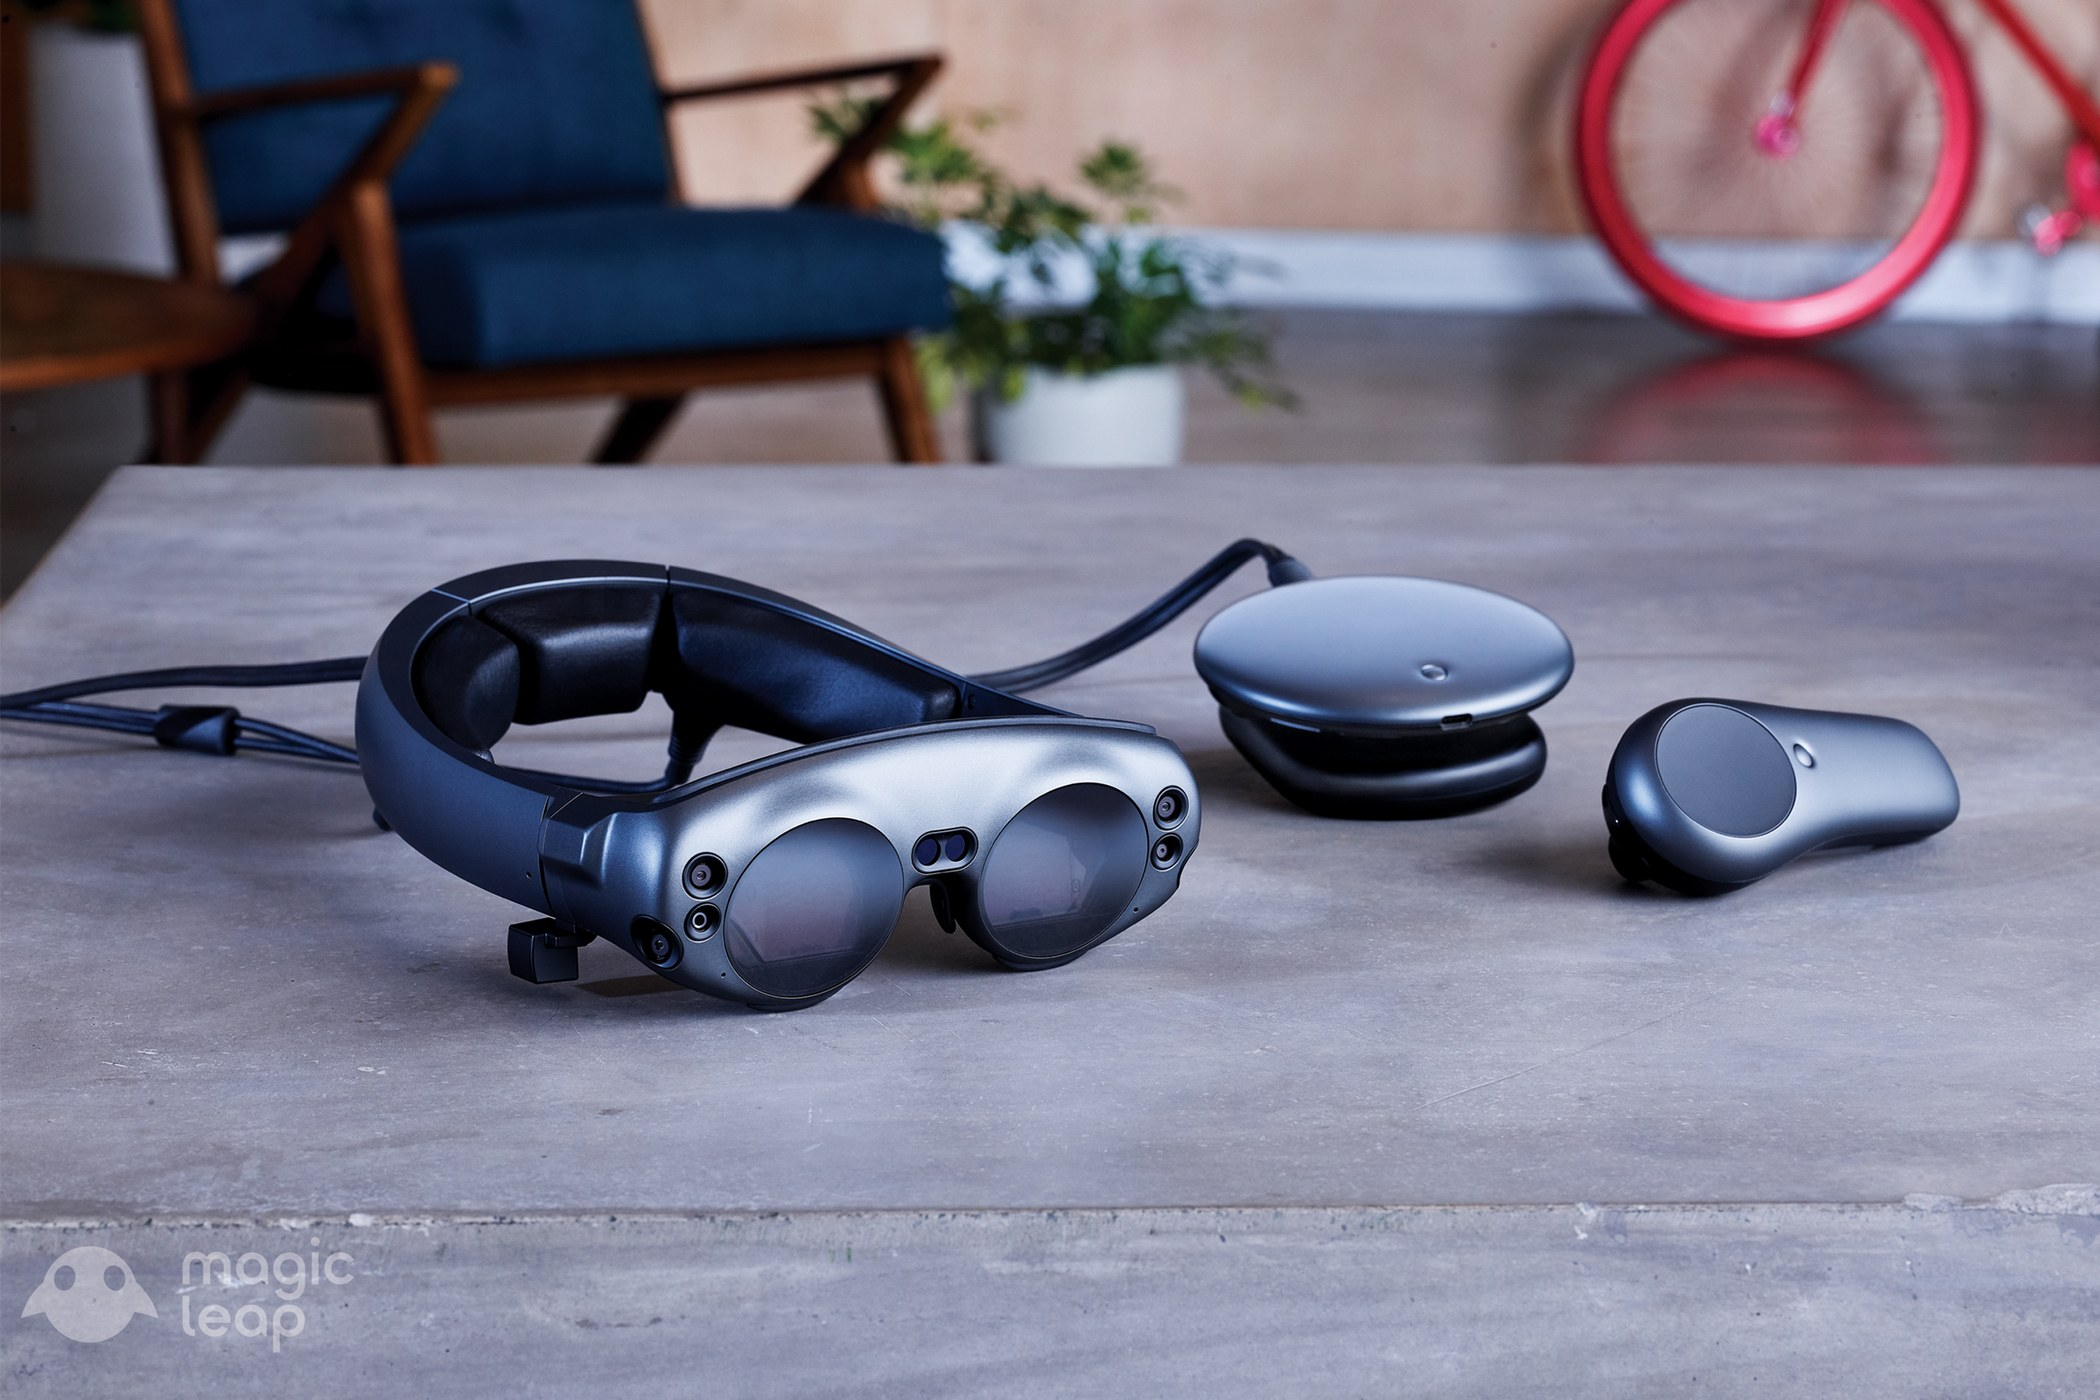
\includegraphics[trim={0, 7cm, 0, 7cm}, clip, width=\textwidth]{figures/magicleap}
    \caption{Das Magic Leap One MR-HMD. \quelle{\cite{MagicLeap2018b}}}
    \label{fig:magic_leap}
\end{figure}

Zu Beginn der Arbeit war das Ziel die Implementierung der Megamap für das Magic Leap One HMD.
Da dieses aber erst im späteren Verlauf der Arbeit veröffentlich wurde, wurde stattdessen die Implementierung für das Vive-HMD in VR umgesetzt.
Die \enquote{reale} Umgebung des Nutzers wird dabei virtuell nachgebildet.
Dadurch lässt sich die Megamap-Anwendung in zukünftigen Arbeiten auf ein MR-HMD übertragen.

%Die Implementierung der Megamap dient der Beantwortung der zentralen Fragestellung dieser Arbeit:
%\begin{quote}
%    \itshape
%    Ist eine in die Umgebung integrierte 3D-Megamap geeignet, um Nutzer bei der Exploration von Gebäuden zu unterstützen?
%\end{quote}
%Der Prototyp wird daher in einer Nutztungsevaluation getestet, um seine Effektivität für die Gebäudeexploration festzustellen.

%Als Inspirationsquelle für die Anwendung dienen neben bereits existierenden Kartenanwendungen wie Google Maps und Ansätzen aus der Forschung auch digitale Spiele.
%Da in Spielen Aufgaben wie Navigation und Exploration von großer Bedeutung sind, kann hier unterschiedliche Ansätze zur Navigations- und Explorationsunterstützung gefunden werden.
%Dies ist am Beispiel TCTD erkennbar.

Da die Idee für die Megamap einem Videospiel entspringt ist nicht unmittelbar klar, ob sich das Konzept auf die Nutzung in der realen Welt übertragen lässt.
Insbesondere, weil die Megamap aus TCTDs Dritte-Person-Perspektive (\emph{Third-Person Perspective}) in die Egoperspektive überführt wird.
Die Eignung der Megamap für die Kartenexploration wird daher am entwickelten Prototypen in einer Nutzerstudie überprüft.
Einerseits werden die subjektiven Eindrücke der Probanden von der Nutzung der Megamap festgehalten.
Andererseits wird die Performance im Vergleich zu einer herkömmlichen 2D-Darstellung einer Indoor-Karte verglichen.

\section{Struktur der Arbeit}
\label{sec:struktur}
Die restliche Arbeit ist in die folgenden Abschnitte unterteilt:

\noindent
Im nächsten Kapitel wird der Stand der Forschung und Technik zur Darstellung von dreidimensionalen Karten beleuchtet.
Die Unterschiede zum Konzept dieser Arbeit sowie deren Beitrag zum Thema werden ebenso herausgearbeitet.
\autoref{chap:concept} geht detailliert auf die Konzeptionierung der 3D-Megamap ein.
Es wird vor allem beschrieben, welche Interaktionen für die Kartenexploration wichtig sind und wie diese in der Megamap-Anwendung umgesetzt werden sollen.
Danach wird in \autoref{chap:implementation} die Implementierung der Anwendung beschrieben.
Ebenso werden Probleme bei der Implementierung erläutert, die für zukünftige Arbeiten beachtet werden sollten.
\autoref{chap:evaluation} präsentiert die Durchführung der Nutzungsevaluation der Anwendung sowie deren Ergebnisse.
Schließlich werden in \autoref{chap:closing} offene Fragen und Probleme dieser Arbeit genannt, welche für zukünftige Arbeiten von Interesse sind.
%
\cleardoublepage

%\chapter{Stand der Forschung}
\label{chap:related_work}

\section{Von Realität bis Virtualität}
Da es sich bei den unten genannten Arbeiten und Systeme um AR-/VR-Anwendungen handelt, müssen vorab die Unterschiede zu herkömmlichen Computerprogrammen und mobilen Applikationen geklärt werden.
Im Folgenden werden die Begriffe \emph{Augmented/Virtual Reality} definiert und ein Überblick der wichtigsten Technologien wird gegeben.

\textcite{Milgram1994} stellen das Konzept eines Kontinuums von Realität zur Virtualität vor (siehe \autoref{fig:rv_kontinuum}).
Anwendungen und Technologien lassen sich dabei in dieses Kontinuum einordnen.
Allgemein werden dabei die Kategorien Augmented Reality, Augmented Virtuality und Virtual Reality unterschieden.

\begin{figure}[h]
    \centering
    \imageframe{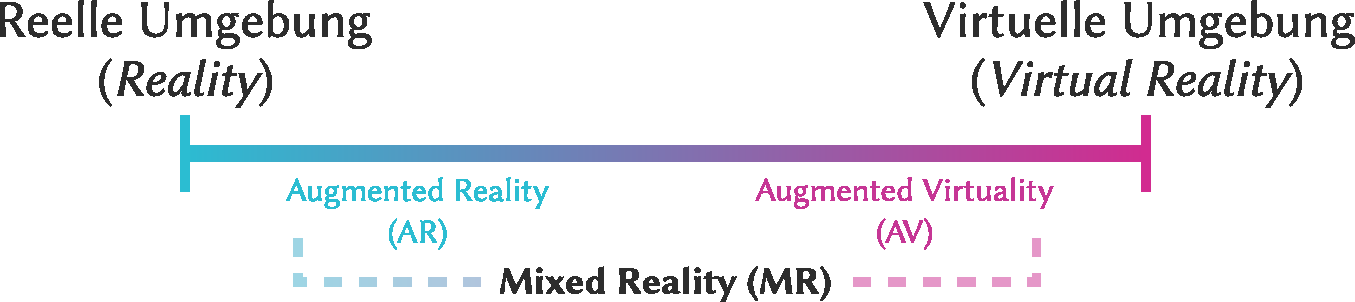
\includegraphics[width=0.9\linewidth]{figures/rv_kontinuum_milgram.pdf}}
    \caption{Das Realität-Virtualität-Kontinuum nach \textcite{Milgram1994}. Je nach Anwendung wird die Realität mehr und mehr mit virtuellen Objekten überlagert, bis schließlich nur noch eine virtuelle Umgebung dargestellt wird.}
    \label{fig:rv_kontinuum}
\end{figure}

Nach \textcite{Azuma1997} bezeichnet \emph{Augmented Reality} Systeme, welche die folgenden Eigenschaften besitzen:
\begin{itemize}
    \item Reale und virtuelle Inhalte werden kombiniert. Häufig werden hierfür virtuelle Objekte auf die reale Umgebung überlagert.
    \item Der Nutzer kann in Echtzeit mit den Systemen interagieren. So zählen z.B. Spezialeffekte in Filmen \emph{nicht} als AR.
    \item Die Inhalte werden dreidimensional mit der Umgebung registriert. Demnach ist ein 2D-Interface vor einer realen Umgebung \emph{kein} AR, selbst wenn es interaktiv ist.
\end{itemize}
AR selbst lässt sich dabei noch in die Kategorien \emph{Spatial AR} und \emph{See-Through AR} einteilen.
Bei Spatial AR werden digitale Informationen direkt in die Umgebung des Nutzers projiziert, z.B. mit einem Projektor auf einen Tisch.
Beim See-Through AR hingegen werden Displays genutzt, die entweder ein Live-Video der Umgebung zeigen oder aber transparent und damit durchsichtig sind.
Dies können See-Through HMDs wie die Microsoft HoloLens sein, aber auch Smartphones in einer entsprechenden HMD-Halterung, bei denen die Rückseitenkamera für ein Live-Bild der Umgebung genutzt wird.
Hier werden die virtuellen Informationen direkt auf dem Display überlagert \autocite{Zachmann2015}.

Bei der \emph{Augmented Virtuality} (AV) werden umgekehrt reale Informationen in eine virtuelle Umgebung eingebettet.
Als Beispiel nennt \textcite[6]{Schroeder2017} die Wetterkarte im Fernsehen, bei der eine \emph{virtuelle} Karte \emph{reale} Wetterinformationen darstellt und um einen \emph{realen} Moderator erweitert wird.
Es sei darauf hingewiesen, dass in diesem Beispiel die Interaktion zwischen dem Moderator und der Karte besteht, nicht etwa zwischen dem Zuschauer und der Karte.

\emph{Virtual Reality} ist die Bezeichnung für Anwendungen, die sich komplett in einer virtuellen Umgebung abspielen.
Um VR von herkömmlichen Computersimulationen abzugrenzen nennt \textcite{Zachmann2015} die intuitive Echtzeit-Interaktion als ein wichtiges Kriterium.
Dabei können Nutzer mit der virtuellen Umgebung über Eingabegeräte wie z.B. Controller mit sechs Freiheitsgraden (6DOF) oder haptischen Eingabegeräten interagieren.
Ein weiteres wichtiges Kriterium ist die Immersion.
Diese ergibt sich aus der Summe der vom System stimulierten und gleichzeitig abgeschirmten Sinne.
Aus diesem Grund werden bei VR-Anwendungen häufig HMDs eingesetzt, da diese gleichzeitig den Sehsinn vor der Außenwelt abschirmen und mit virtuellen Bildern stimulieren können.
% TODO: Links zu den Displayarten.
Aber auch halb-immersive Displays wie eine \emph{Cave}, eine \emph{Powerwall} oder ein Volumendisplay sind möglich.

\textcite{Milgram1994} nennen ebenfalls den Begriff der \emph{Mixed Reality} (MR).
Dieser wird in der Literatur als Oberbegriff sowohl für AR als auch AV verwendet.
Der Begriff hebt die Kombination von realen und virtuellen Inhalten hervor.

\section{Augmentierte Navigation}
Bereits \textcite{Hoellerer1999} stellen ein AR-System vor, bei dem zwei Nutzer kooperieren können.
Der eine Nutzer bewegt sich zu Fuß mit einem HMD und einem Tablet-Computer in der Außenwelt.
Durch das HMD können ihm augmentierte Informationen zur Umgebung und sogar ganze virtuelle Gebäude dargestellt werden, die mit der Umgebung registriert sind.
Der andere Nutzer kann entweder über ein Desktop-Interface oder eine AR-Darstellung der Karte Routen und Informationen in der Umgebung platzieren.
Damit stellt diese Arbeit eine frühe Implementierung für ein HMD dar, die sowohl Navigations- als auch Explorationsaufgaben unterstützt.

Wie bereits in \autoref{sec:motivation_ziel} erwähnt fokussiert sich ein großer Teil der bisherigen Forschung auf den Usecase der Navigation von einem Punkt zu einem anderen.
Vor allem das AR-unterstützte Autofahren wird betrachtet, da hier eine fehlerfreie Navigation wichtig ist und im Fehlerfall sogar fatale Folgen haben kann \parencite{Lin2017}.
Ein häufig eingesetztes Mittel ist hier die virtuelle Hervorhebung der Straßenführung.
\textcite{Narzt2006} präsentieren ein allgemeines Framework zur Darstellung einer virtuellen Route.
Das Framwork kann sowohl für Fahrzeug- als auch Fußgängernavigation und auf verschiedenen Endgeräten eingesetzt werden.
Für den Einsatz im Auto schlagen die Autoren die Windschutzscheibe als Display vor.
Dadurch wäre das AR-Display in der natürlichen Umgebung des Nutzers integriert.
\textcite{Bark2014} erweitern diesen Ansatz.
Sie ersetzen in einem zuvor aufgenommenen Video die statische virtuelle Route durch eine Reihe animierter Papierflieger, die entlang der geplanten Route fliegen.
\textcite{Kim2009} ersetzen die Route sogar durch eine 2.5D-Karte mithilfe eines Fahrsimulators.
Von der Oberseite der Windschutzscheibe schiebt sich eine 2D-Karte ins Sichtfeld, die sich nach und nach dreidimensional mit der Straße verbindet.
Bei beiden Ansätzen wiesen die Autoren beim Vergleich mit einem herkömmlichen \emph{top-down} GPS-System nach, dass die Probanden dem Straßenverlauf durch die AR-Unterstützung besser folgen konnten und weniger Fehler bei der Navigation machten.

\textcite{Alnabhan2014} präsentieren einen Ansatz zur \emph{Indoor}-Navigation als \emph{Android-App}.
Die App nutzt \emph{\wifi-Fingerprinting} und den digitalen Kompass eines Smartphones/Tablets zur Positionierung und Orientierung.
Über vordefinierte Referenzpunkte im Gebäude wird die Ungenauigkeit des \wifi-Fingerprintings ausgeglichen.
Navigationshinweise werden als AR-Pfeil angezeigt (mit zusätzlichen Textausgaben).
Alternativ dazu zeigen \textcite{Liu2016} einen ähnlichen Ansatz, bei dem die Positionierung jedoch auf Magnetfeldsensoren aufbaut und daher weder auf GPS noch auf Infrastruktur wie \wifi oder Marker angewiesen ist.
% TODO: Diesen Satz anpassen, je nachdem wie die Entwicklung der Megamap ausgeht.
Das zeigt, dass AR-unterstützte Kartenanwendungen durchaus auch innerhalb von Gebäuden umsetzbar sind.

\section{Digitale Kartenexploration}
Zur AR-Exploration tragen \textcite{Reitmayr2005} bei, indem sie eine reale Papierkarte durch einen Projektor augmentieren.
\autoref{fig:reitmayr2005_helicopter_map} zeigt die Funktionsweise.
Ein projizierter Helikopter kann mit einem realen \emph{Personal Digital Assistant} (PDA) bewegt werden, wenn dieser in die Nähe gehalten wird.
Der PDA zeigt währenddessen ein Interface zur Kontrolle des Helikopters.
Der Helikopter dient als Cursor für kontextbasierte Informationen.
Sobald der Nutzer einen Rahmen auf die Karte legt, projiziert der Projektor ein Bild der aktuellen Kartenposition aus ungefährer Sicht des Helikopters auf ihn.
Zudem kann der Zustand der Karte durch die Projektion dynamisch verändert werden (in diesem Fall werden Gezeiten von Gewässern simuliert).
Auch wenn diese Arbeit nicht für einen mobilen Einsatz geeignet ist, wird deutlich, dass mit AR nicht nur ortsbezogene sondern auch zeitbezogene Daten auf einer Karte dargestellt werden können.
Dies erlaubt also zusätzlich eine Exploration in der zeitlichen Dimension einer Karte.

\begin{figure}[h]
    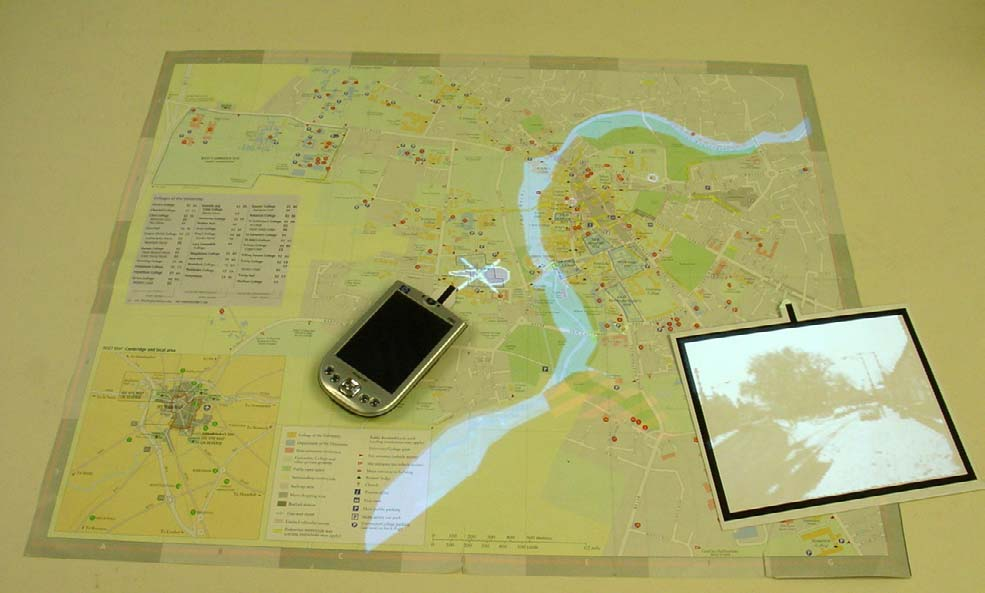
\includegraphics[width=\textwidth]{figures/reitmayr2005_helicopter_map.png}
    \caption{Eine reale Papierkarte wird durch einen Projektor mit virtuellen Inhalten angereichert. \quelle{\cite{Reitmayr2005}}}
    \label{fig:reitmayr2005_helicopter_map}
\end{figure}

\section{Virtuelle Umgebungen als World-in-Miniature}
% WIM
Die Idee der Megamap ist im Prinzip, ein herunterskaliertes Abbild der Umgebung um den Nutzer zu platzieren.
Damit ist die Megamap eine Variante der World-in-Miniature-Metapher (WIM).
Dies ist ein Ansatz zur Unterstützung von Navigation und Interaktion, der vor allem in virtuellen Welten Anwendung findet.
Dabei wird die nähere Umgebung miniaturisiert dargestellt und häufig als eigenständiges Objekt vom Nutzer in der Hand gehalten.
Je nach Anwendung ergeben sich hieraus unterschiedliche Interaktionsmöglichkeiten \parencite{Stoakley1995}.

\textcites{Mulloni2011a}{Mulloni2012} nutzen einen kombinierten Ansatz aus AR-Hinweisen und WIM.\@
Während Nutzer durch ein Gebäude navigieren werden AR-Pfeile sowie Navigationsanweisungen in Form von \enquote{Aktivitäten} auf einem Smartphone angezeigt (\autoref{sfig:mulloni2011_wim_b}, \subref{sfig:mulloni2011_wim_e}).
Sobald zuvor platzierte Poster an Infopunkten im Gebäude erreicht und gescannt werden, wechselt die Ansicht zu einer WIM-Darstellung der Etage mit der hervorgehobenen Route zum Zielort (\autoref{sfig:mulloni2011_wim_a}, \subref{sfig:mulloni2011_wim_c}, \subref{sfig:mulloni2011_wim_d}).
Laut dem Ergebnis der Studie der Autoren hilft die WIM-Übersicht den Nutzern, gewisse Orientierungspunkte (\emph{\enquote{Landmarks}}) in der Umgebung wiederzuerkennen, was zu weniger Fehlern bei der Navigation führt.
Von diesem Aspekt könnte auch die Megamap profitieren, welche eine WIM-ähnliche Sicht der näheren Umgebung liefert.

\begin{figure}[h]
    \begin{subfigure}{.195\textwidth}
        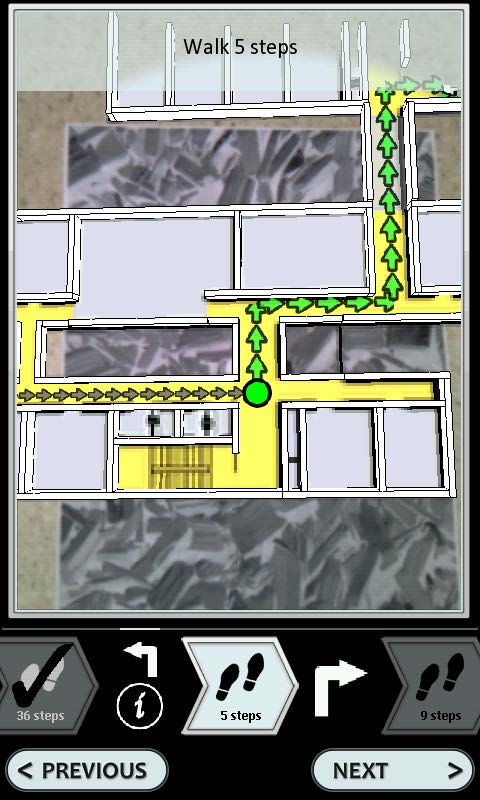
\includegraphics[width=\textwidth]{figures/mulloni2011_wim_a.png}
        \caption{}
        \label{sfig:mulloni2011_wim_a}
    \end{subfigure}
    \hfill
    \begin{subfigure}{.195\textwidth}
        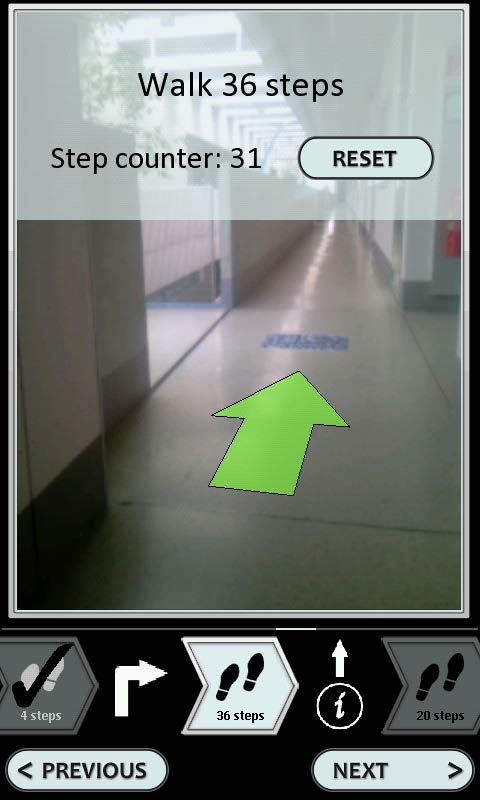
\includegraphics[width=\textwidth]{figures/mulloni2011_wim_b.png}
        \caption{}
        \label{sfig:mulloni2011_wim_b}
    \end{subfigure}
    \hfill
    \begin{subfigure}{.195\textwidth}
        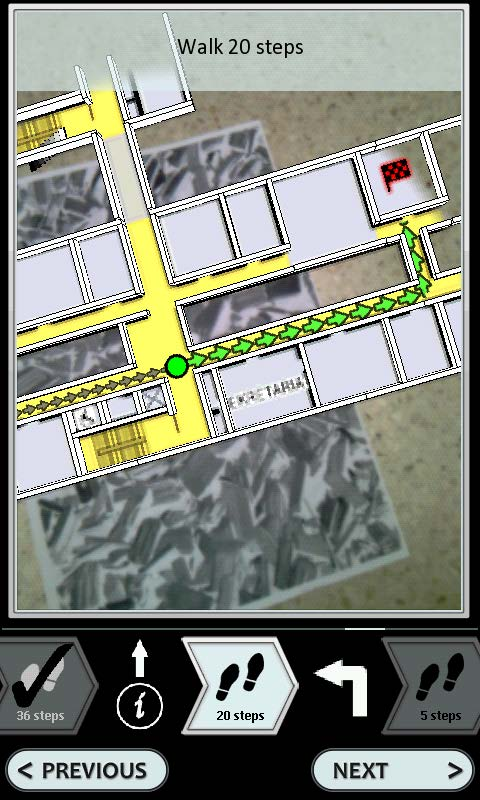
\includegraphics[width=\textwidth]{figures/mulloni2011_wim_c.png}
        \caption{}
        \label{sfig:mulloni2011_wim_c}
    \end{subfigure}
    \hfill
    \begin{subfigure}{.195\textwidth}
        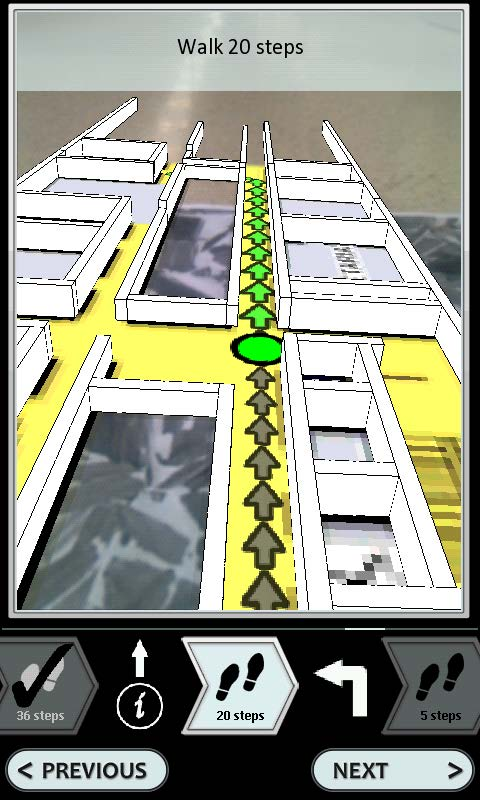
\includegraphics[width=\textwidth]{figures/mulloni2011_wim_d.png}
        \caption{}
        \label{sfig:mulloni2011_wim_d}
    \end{subfigure}
    \hfill
    \begin{subfigure}{.195\textwidth}
        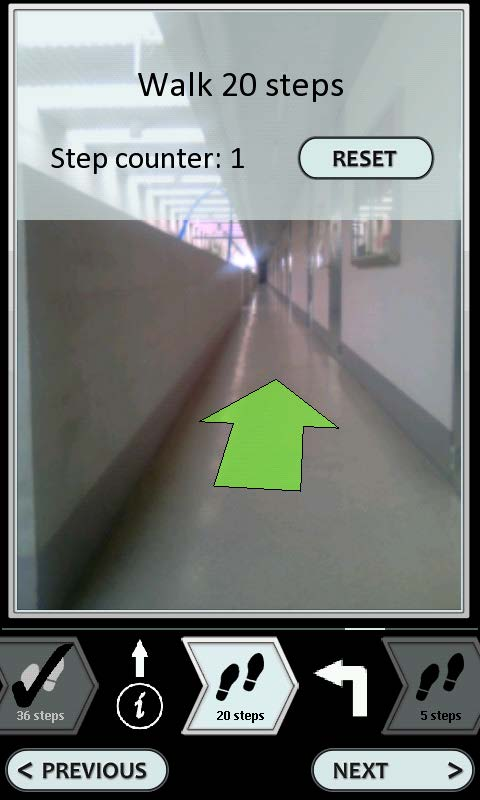
\includegraphics[width=\textwidth]{figures/mulloni2011_wim_e.png}
        \caption{}
        \label{sfig:mulloni2011_wim_e}
    \end{subfigure}
    \caption{AR-Interface für Indoor-Navigation basierend auf WIM.\@ An den Lokalisierungspunkten wird die Indoor-Karte als WIM angezeigt und mit der Position/Rotation der Umgebung registriert. \quelle{\cite{Mulloni2011}}}
    \label{fig:mulloni2011_wim}
\end{figure}

\textcite{Chittaro2005} erweitern das Konzept von WIM für mehrstöckige Gebäude als eine \emph{BreakAway}-Karte (\autoref{fig:chittaro2005_breakaway}).
Hier können einzelne Stockwerke zur Seite geschoben und ausgeblendet werden, um so auf Stockwerke blicken zu können, auf denen sich der Nutzer selbst gar nicht befindet.
Dies erleichtert die Exploration von Gebäuden, da diese schneller nach den gewünschten Eigenschaften durchsucht werden können.

\begin{figure}[h]
    \begin{subfigure}{.49\textwidth}
        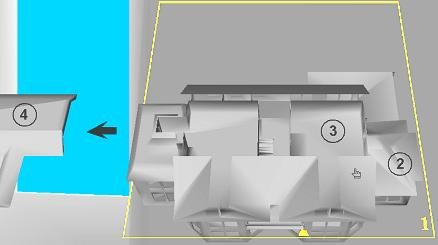
\includegraphics[width=\textwidth]{figures/chittaro2005_breakaway_a.png}
%        \caption{}
    \end{subfigure}
    \hfill
    \begin{subfigure}{.49\textwidth}
        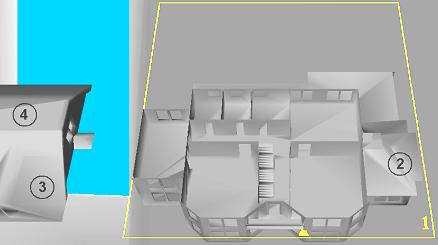
\includegraphics[width=\textwidth]{figures/chittaro2005_breakaway_b.png}
%        \caption{}
    \end{subfigure}
    \caption{In der \emph{\enquote{Examine View}} der BreakAway-Karte können Stockwerke zur Seite geschoben werden, um den Blick auf darunterliegende Stockwerke zu ermöglichen. \quelle{\cite{Chittaro2005}}}
    \label{fig:chittaro2005_breakaway}
\end{figure}

\textcite{Vallance2001} schlagen zudem eine Krümmung der WIM-Umgebung vor, um so eine Verdeckung durch Wände und andere Objekte zu minimieren.

\section{Kartenexploration in digitalen Spielen}
% TODO Übergang?
Im Bereich der Video- und Computerspiele untersuchen \textcites{Moura2014}{Moura2015} den Zusammenhang zwischen eingesetzten Navigationshelfern, Design der Level, sowie Spielmechaniken zur Unterstützung der Navigation.
Daraus leiten \textcite{Moura2015} eine Klassifikation von Navigationshelfern ab.
Außerdem erstellen sie eine Liste von Design-Richtlinien, welche die Vor- und Nachteile der jeweiligen Helfer erläutern und als Hilfestellung für Entwicklung von neuen Spielen dienen.
Diese Designrichtlinien werden in die Entwicklung der Megamap mit einbezogen.

Aufbauend auf die Navigationshelfer in Spielen untersucht \textcite{Lodts2015}, ob diese Helfer auch in der realen Welt anwendbar sind.
Dazu wurden unterschiedliche Helfer, wie sie aus Spielen bekannt sind, für das \emph{Google Glass} implementiert.
In einem Test, aufgeteilt in die Aufgabenbereiche Navigation, Orientierung, Exploration und Annotation, wurde ermittelt welche der Helfer den Nutzern bei der jeweiligen Aufgabe am hilfreichsten sind.
Es zeigt sich, dass Helfer, die in der Umgebung eingebettet sind (z.B. AR-Pfeile oder -Text, farbliche Hervorhebungen von Objekten) effektiver sind als statische Anzeigen per \emph{Head-Up Display} (HUD).
Daher wird bei der Entwicklung der Megamap-Anwendung der AR-Darstellung von Inhalten mehr Beachtung geschenkt.
%
\cleardoublepage
%\include{...}
\chapter{Implementierung}
\label{chap:implementation}
\begin{figure}[h!]
    \centering
    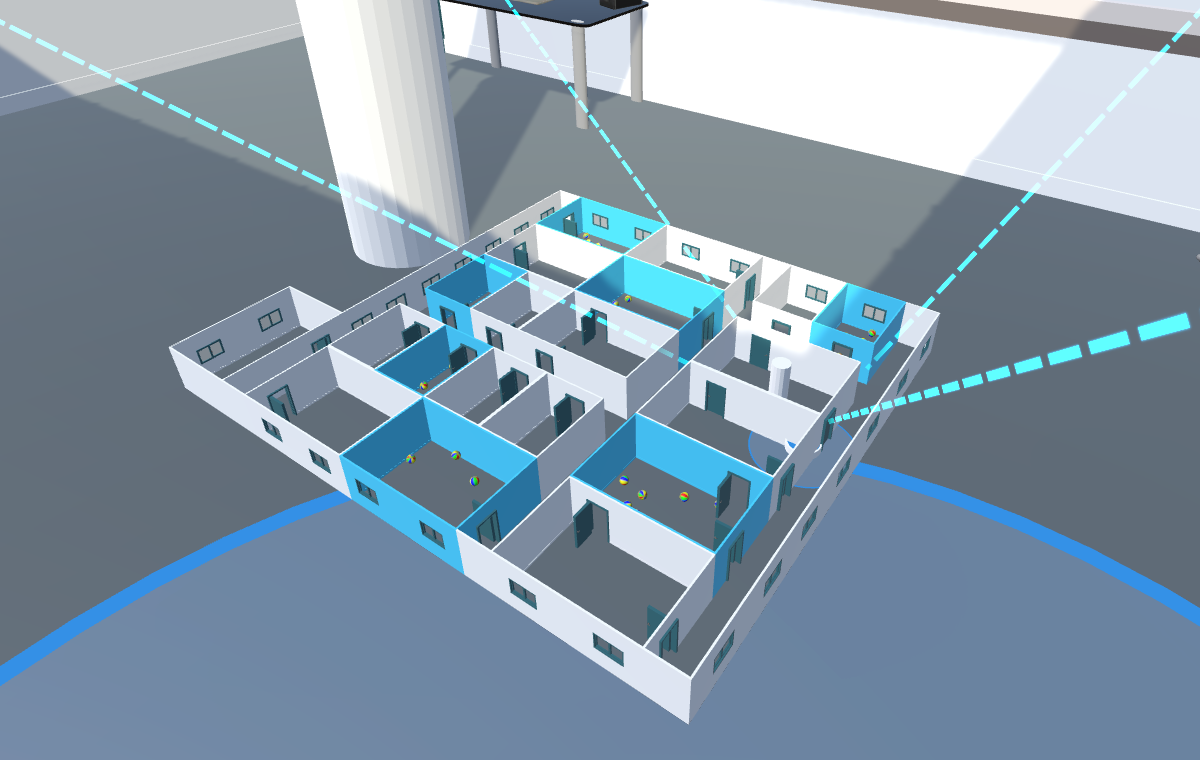
\includegraphics[width=\linewidth]{figures/screenshots/condition_3d_l_x}
    \caption{Beispiel des finalen Megamap-Prototypen in der Übersicht.}
    \label{fig:megamap_overview}
\end{figure}

\section{Unity Engine}
\emph{Unity} \autocite{UnityTechnologies2018} ist eine \emph{Engine} zum Entwickeln von 2D- und 3D-Anwendung (vornehmlich Spiele).
Da Unity plattformunabhängig ist werden die Applikationen gleichzeitig für mehrere Plattformen entwickelt.
Erstellt werden die Anwendungen mit dem Unity Editor.

Eine Unity-Anwendung ist in Szenen unterteilt.
Jede Szene besitzt einen eigenen Szenengraph.
Dieser Graph verwaltet alle Objekte einer Szene.
Unity verwendet ein Entitäten-Komponenten-System.
Das heißt, alle Unity-Objekte sind im Kern attribut- und funktionslose Entitäten (in Unity \emph{GameObject}s genannt).
Die eigentliche Funktionalität wird erst durch Hinzufügen von Komponenten (\emph{Components}) zu den GameObjects deutlich.
Beispielsweise verfügt das GameObject eines Würfel-Objekts über die Komponenten \lstinline{Transform} (Position, Rotation und Skalierung), \lstinline{MeshRenderer} (Geometrie) und \lstinline{BoxCollider} (Kollision).
Neben Anwendungen für den Desktop oder mobile Endgeräte bietet Unity native Unterstützung für eine Vielzahl an AR- und VR-Plattformen an \parencite{UnityTechnologies2018b}.

Zusätzlich zu diesen vorgefertigten Komponenten können auch Skript-Komponenten zu den GameObjects hinzugefügt werden.
Dies ermöglicht Entwicklern, komplett neues Verhalten für Objekte in die Engine zu integrieren.
Die Skripte werden in C\# oder einem Javascript-Dialekt geschrieben.
Die Skripte erben von der Unity-Klasse \lstinline|MonoBehaviour|, wodurch sie in den Lebenszyklus von Unity-Objekten aufgenommen werden und Eventmethoden wie z.B. \lstinline|Start()|, \lstinline|Update()|, \lstinline|FixedUpdate()| usw. erhalten \parencite{UnityTechnologies2018c}.

Eine Besonderheit bei Unity im Vergleich zu anderen Engines sind die \emph{Prefabs}.
Dabei handelt es sich um abgespeicherte Konfigurationen von GameObjects inklusive derer Komponenten.
Die Prefabs können dann jederzeit als vorkonfiguriertes Objekt instanziiert werden.
Darüber hinaus lässt sich Unity durch das Importieren von Plugins erweitern.
So werden \emph{Assets} (Texturen, Fonts, Musik, Materialien, Skripte) und Prefabs von anderen Entwicklern in das aktuelle Projekt übernommen.
Aufgrund der einfach zu nutzenden AR-/VR-Funktionalität sowie der Erweiterbarkeit wird Unity für diese Arbeit eingesetzt.

\section{SteamVR Plugin}
Ein nennenswertes Plugin, was für diese Arbeit eingesetzt wird, ist das \emph{SteamVR Plugin} \autocite{ValveCorporation2018}.
Dieses baut die in Unity integrierte AR-/VR-Unterstützung weiter aus.

Eine zentrale Rolle nimmt das \emph{Player}-Prefab ein.
Durch Platzieren dieses Prefabs in der Unity-Szene werden automatisch GameObjects erzeugt, welche die Positionen und Rotationen vom HMD und weiteren Controllern eines verbundenen VR-Systems tracken.
Die Zuordnung der Geräte zu den GameObjects ist hardware-übergreifend und geschieht automatisch.
Zudem wird dem Nutzer eine Begrenzung des Spielebereichs angezeigt, welche sich aus der verwendeten Technologie ergibt (in diesem Fall die sationären \emph{Lighthouse} Basisstationen der Vive).
Ebenso werden 3D-Modelle der Hand angezeigt, wobei sich die Finger der virtuellen Hände zu den Knöpfen bewegen, die der Nutzer aktuell betätigt.
Das Prefab übernimmt außerdem das stereoskopische Rendern, sodass auf dem HMD für jedes Auge ein anderes Bild angezeigt wird, wodurch der Eindruck von räumlicher Tiefe entsteht.

Für diese Arbeit wird außerdem das \lstinline{Interactable}-SteamVR-Skript verwendet.
Durch dieses Skript können GameObjects mit einer \lstinline{Collider}-Komponente auf die virtuellen Hände bzw. Controller reagieren und interaktive gemacht werden (z.B. Aufnehmen und werfen von Objekten, anklicken von Knöpfen etc.).
Die Verwendungen dieses Skripts für den Megamap-Prototypen werden an entsprechender Stelle in den folgenden Abschnitten näher beschrieben.

\section{Virtuelle Laborumgebung}
Wie eingangs in \autoref{sec:motivation_ziel} erwähnt war die ursprüngliche Idee dieser Arbeit die Implementierung eines Megamap-Prototypen für das MR-HMD Magic Leap One.
Dabei sollte die virtuelle Karte mithilfe des HMDs in die reale Umgebung des Nutzers integriert werden.

Zu Beginn der Arbeit war allerdings statt der MR-Hardware nur ein Software-Simulator als Entwicklervorschau verfügbar.
Im Verlauf der Arbeit wurde die MR-Hardware veröffentlicht.
Das HMD war in der Arbeitsgruppe Human-Computer~ Interaction der Universität Bremen jedoch weiterhin nicht verfügbar.
Daher wurde in dieser Arbeit ein alternativer Prototyp für das VR-HMD HTC Vive entwickelt.
Wie die meisten VR-HMDs verdeckt die Vive das Sichtfeld des Nutzers komplett, um stattdessen die virtuellen Inhalte anzuzeigen.
Somit ist die reale Welt für die Nutzer nicht mehr sichtbar, was die visuelle Integration der Megamap in Umgebung unmöglich macht.

Der entwickelte Prototyp umgeht dieses Problem, indem ein virtuelles Modell der Umgebung im Maßstab 1:1 verwendet wird.
So wird die reale Welt um den Nutzer herum virtuell simuliert.
Die virtuelle Megamap kann dann in die \textit{virtuelle} Umgebung des Nutzers integriert werden.
Die Idee hinter diesem Ansatz ist, dass durch die Ähnlichkeit der realen und der virtuellen Umgebung das Prinzip des VR-Prototypen auf eine Situation mit einem MR-HMD weiterhin übertragbar ist.
In zukünftigen Arbeiten könnte damit der Megamap-Prototyp auf MR-HMDs eingesetzt werden, ohne grundlegende Änderungen vornehmen zu müssen.
Durch die Verwendung eines 3D-Modells wird außerdem die 3D-Rekonstruktionsfunktion der Magic Leap One nachgeahmt.
Wie auch die HoloLens erstellt die Magic Leap One durch aktives Tracking der Umwelt intern ein 3D-Modell der Umgebung.
Dieses wird für die Kollisionsberechnung mit den virtuellen Inhalten verwendet.
So können virtuelle Objekte mit realen Gegenständen interagieren (z.B. läuft ein Charakter über einen realen Tisch oder ein virtueller Bildschirm wird an einer realen Wand platziert).
Durch die Verwendung eines 3D-Modells der Umgebung im Megamap-Prototypen ist Möglichkeit der Interaktion mit der Umwelt implizit gegeben.

Für den Prototypen wurde ein maßstabsgetreues 3D-Modell des Laborraums der Arbeitsgruppe Human-Computer~ Interaction der Universität Bremen angefertigt, welcher der Ort der durchgeführten Nutzerstudie ist (siehe \autoref{chap:evaluation}).
\autoref{fig:lab_environment} zeigt ein Foto des Laborraums sowie Screenshots der entsprechenden virtuellen Umgebung.
Der Grundriss des Raums wurde im Modellierungsprogramm \emph{Blender} mithilfe des eingebauten \emph{Archimesh}-Werkzeugs zentimetergenau erstellt.
Das Modell wurde als \texttt{.fbx} in Unity importiert und mit diversen virtuellen Requisiten ergänzt, um den Raum realistischer und dem Original ähnlicher wirken zu lassen.
\begin{figure}[thb]
    \begin{subfigure}{0.49\textwidth}
        \centering
        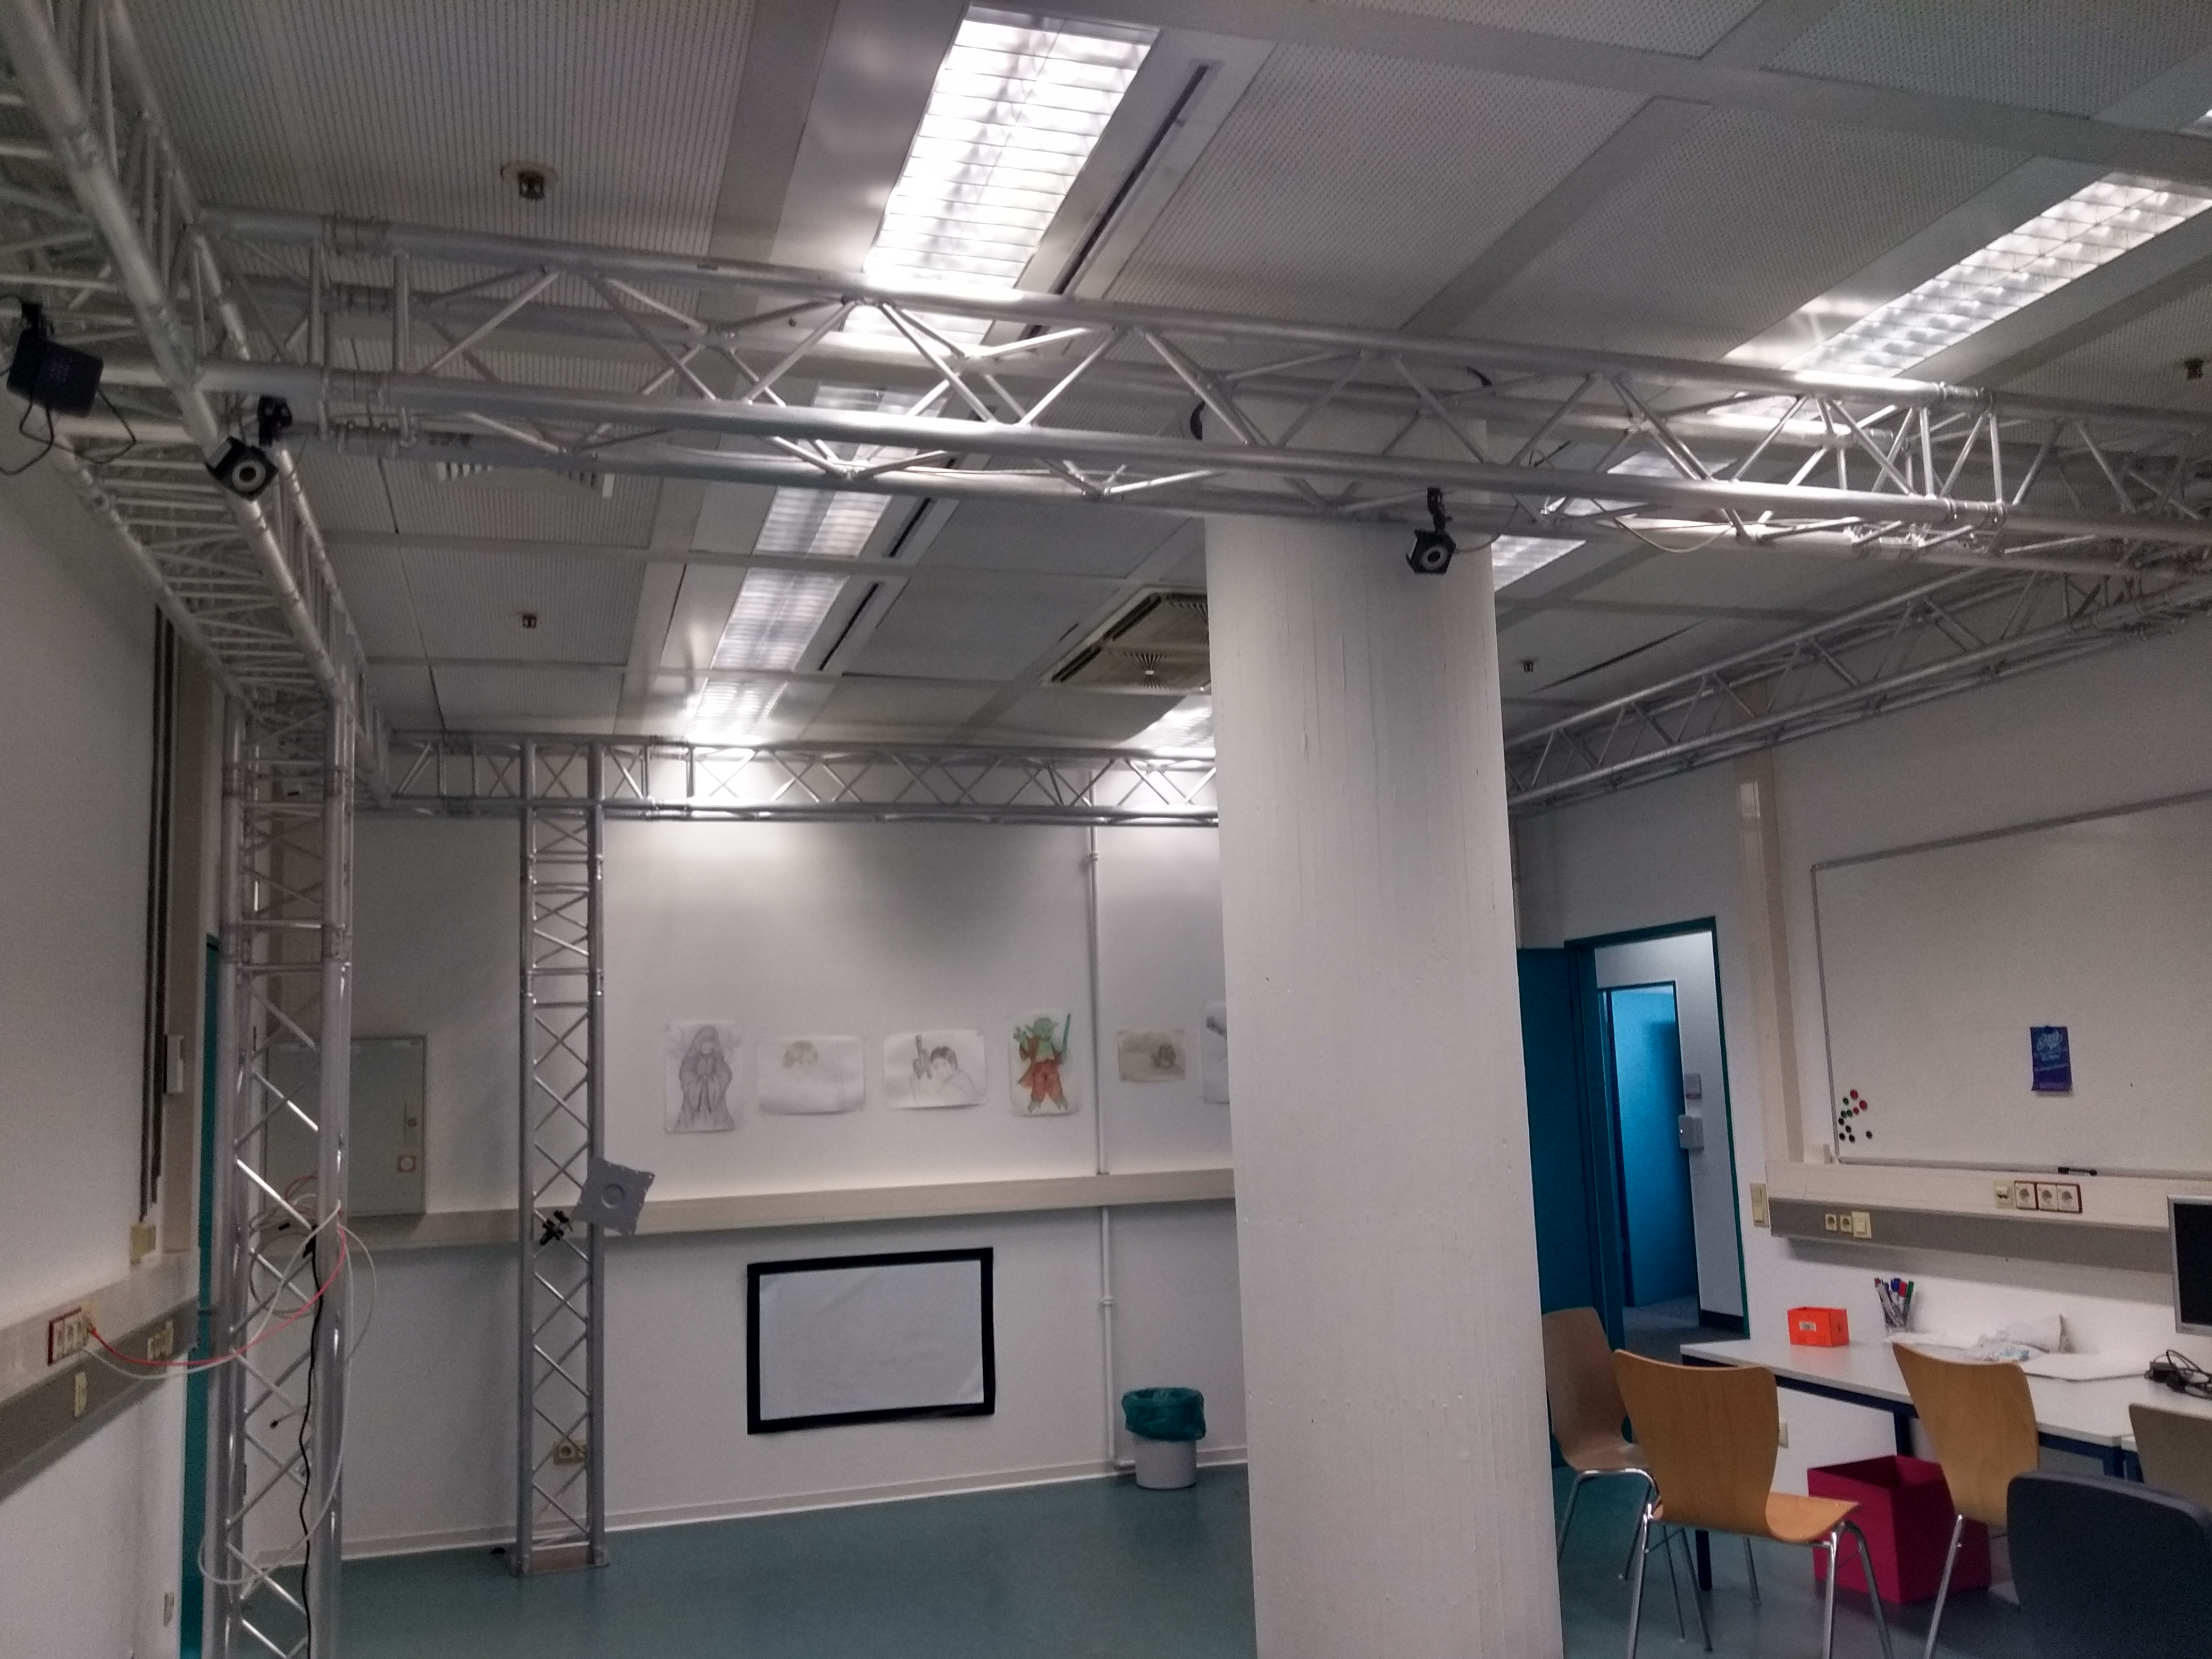
\includegraphics[width=0.755\textwidth]{figures/photo_lab}
        \caption{}
        \label{sfig:lab_photo}
    \end{subfigure}
    \hfill
    \begin{subfigure}{0.49\textwidth}
        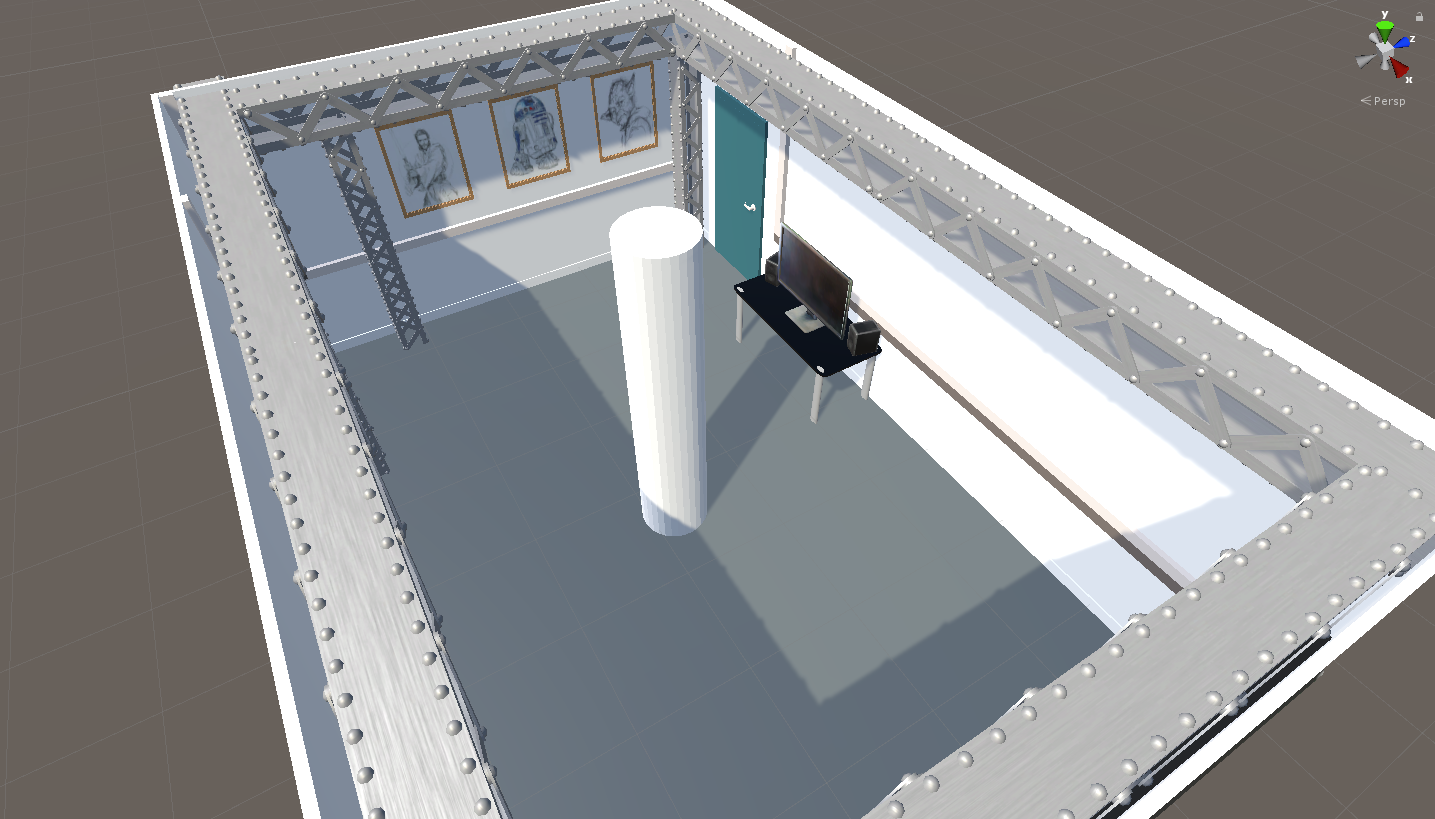
\includegraphics[width=\textwidth]{figures/lab3}
        \caption{}
        \label{sfig:lab_screenshot_1}
    \end{subfigure}

    \vspace{1em}
    \begin{subfigure}{0.49\textwidth}
        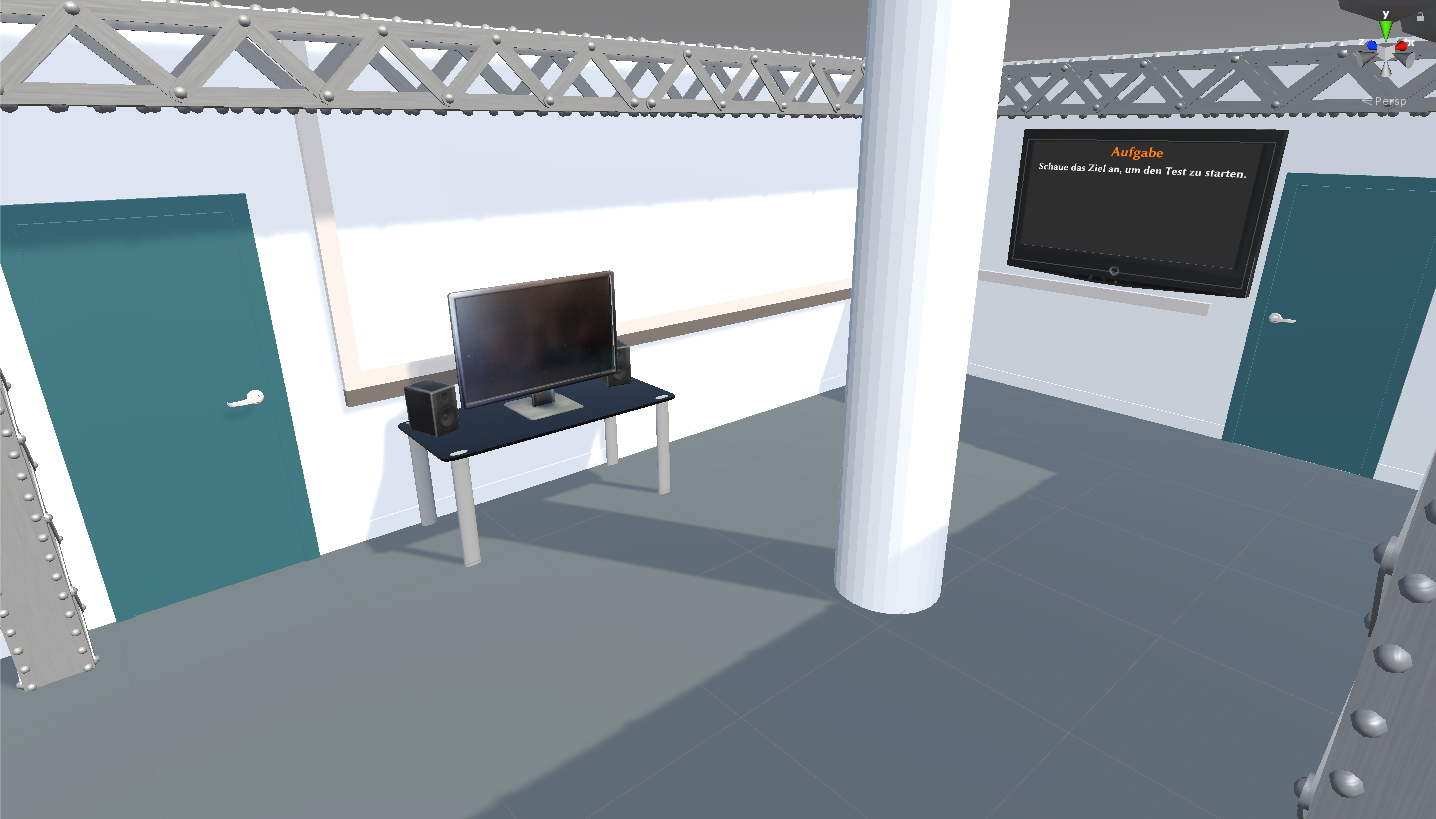
\includegraphics[width=\textwidth]{figures/lab1}
        \caption{}
        \label{sfig:lab_screenshot_2}
    \end{subfigure}
    \hfill
    \begin{subfigure}{0.49\textwidth}
        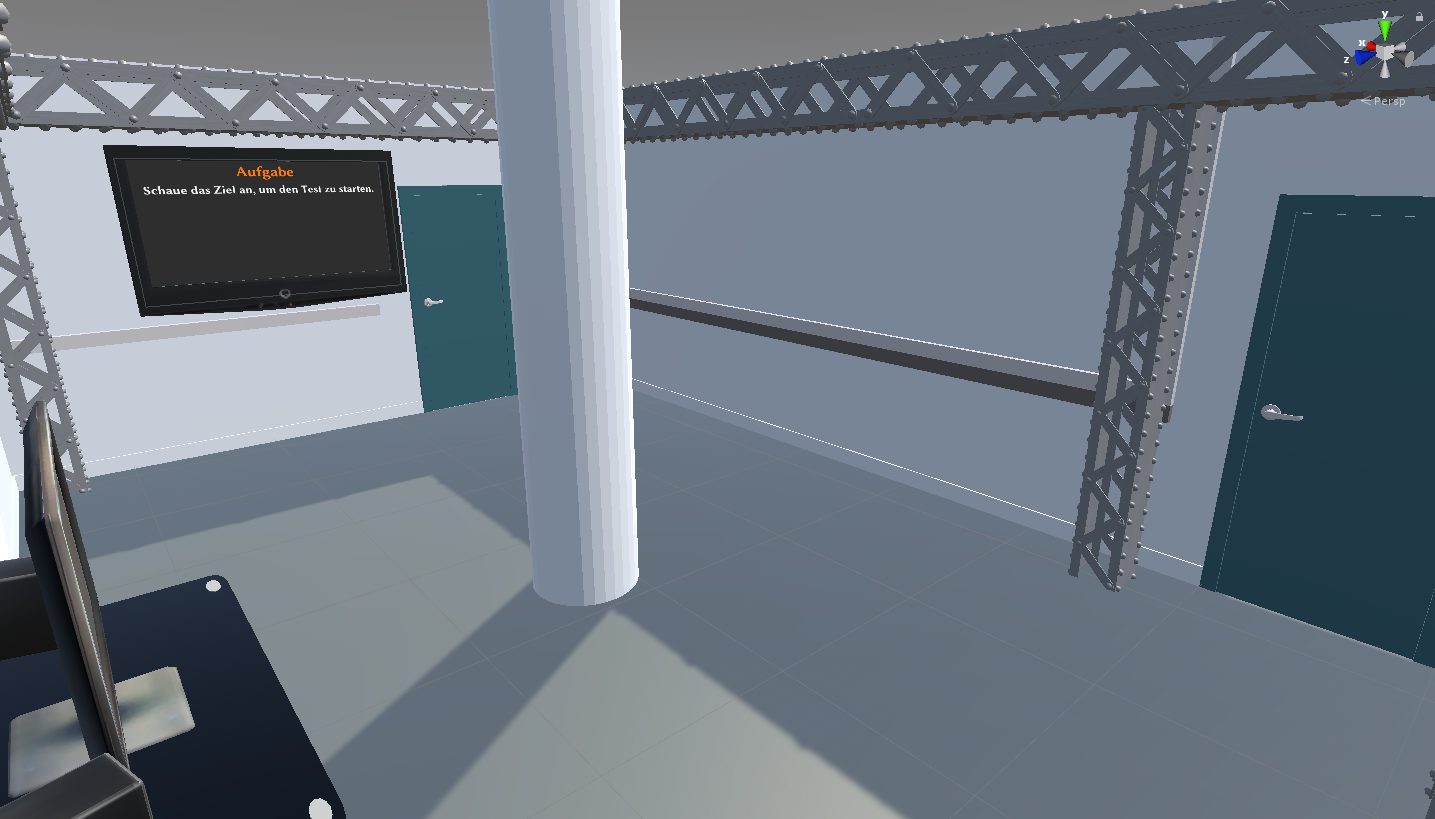
\includegraphics[width=\textwidth]{figures/lab2}
        \caption{}
        \label{sfig:lab_screenshot_3}
    \end{subfigure}
    \caption{Um die Situation der MR-Anwendung in VR nachzubilden, wurde der Laborraum im Maßstab 1:1 modelliert. %
             (\subref{sfig:lab_photo}) Foto des realen Laborraums. %
             (\subref{sfig:lab_screenshot_1})--(\subref{sfig:lab_screenshot_3}) Screenshots des virtuellen Laborraums in Unity.%
	}
	\label{fig:lab_environment}
\end{figure}

\subsection*{Synchronisation der realen und virtuellen Position}
Damit die virtuelle Umgebung als Ersatz für die reale Umgebung verwendet werden kann muss sichergestellt werden, dass die Rotation des virtuellen Raums der des realen Raums entspricht \emph{und} dass die Position des Nutzers in der virtuellen Welt seiner Position in der realen Welt entspricht.
Der Prototyp muss dafür vorab in zwei Schritten konfiguriert werden:

\paragraph{Erster Schritt:}
Während der Kalibrierung der Vive legt der Nutzer den Spielebereich (die sogenannte \emph{Play Area}) fest.
Dies ist der Bereich, in dem sich keine Hindernisse für den Nutzer befinden und der für die Basisstationen sichtbar ist.
Hierfür zieht der Nutzer mit den Controllern ein Rechteck nach, welches dann als Spielebereich gesetzt wird.
Es wichtig, dass die längere Seite des Rechtecks orthogonal zur Ausgangsrotation des \lstinline{Player}-Objekts in Unity verläuft.
Die aktuell getrackte Rotation des HMDs wird relativ zur Ausrichtung der Play Area gemessen.
Da SteamVR automatisch die längeren Seiten der Play Area als Vorder- bzw. Rückseite betrachtet, müssen diese orthogonal zur Blickrichtung des \lstinline{Player}-Objekts verlaufen.
Im Fall des entwickelten Prototypen bedeutet dies, dass die Vorderseite der Play Area parallel zu der Wand des Labors verlaufen muss, an der sich die Eingangstür und Tische befinden (siehe \autoref{fig:lab_environment}).
Die korrekte Kalibrierung der Play Area wird in \autoref{fig:ve_setup_correct} skizziert.
Wenn bei der Kalibrierung der Play Area eine andere Ausrichtung gewählt wird, als die Ausgangsrotation des \lstinline{Player}-Objekts, weicht die virtuelle Rotation des Nutzers von der realen Rotation im Bezug zum Raum ab.
Effektiv hätte die virtuelle Umgebung dann eine andere Ausrichtung als die reale Umgebung.
Die falsche Kalibrierung wird in \autoref{fig:ve_setup_wrong} dargestellt.

Ginge es nur um den visuellen Reiz in der virtuellen Umgebung, würde der Nutzer diese Abweichung lediglich beim Aufsetzen des HMDs bemerken (da dann der virtuelle Raum anders rotiert wäre als der reale).
Wenn aber zum Beispiel der Tastsinn eine Rolle spielt, dann ist eine korrekte Ausrichtung des virtuellen Raums sinnvoll.
Da in dem entwickelten Prototyp nicht ausgeschlossen ist, dass der Nutzer die Play Area verlässt und beispielsweise die Säule oder Wände mit den Händen berührt, ist es für die Immersion von Vorteil, wenn das Berühren der virtuellen Objekte mit den taktilen Reizen der realen Objekte verknüpft wird.
Weiterhin wird durch die korrekte Ausrichtung die Messung des Abweichungsfehlers beim Zeigen auf Objekte erleichtert, was detailliert in \autoref{chap:evaluation} beschrieben wird.

\begin{figure}
    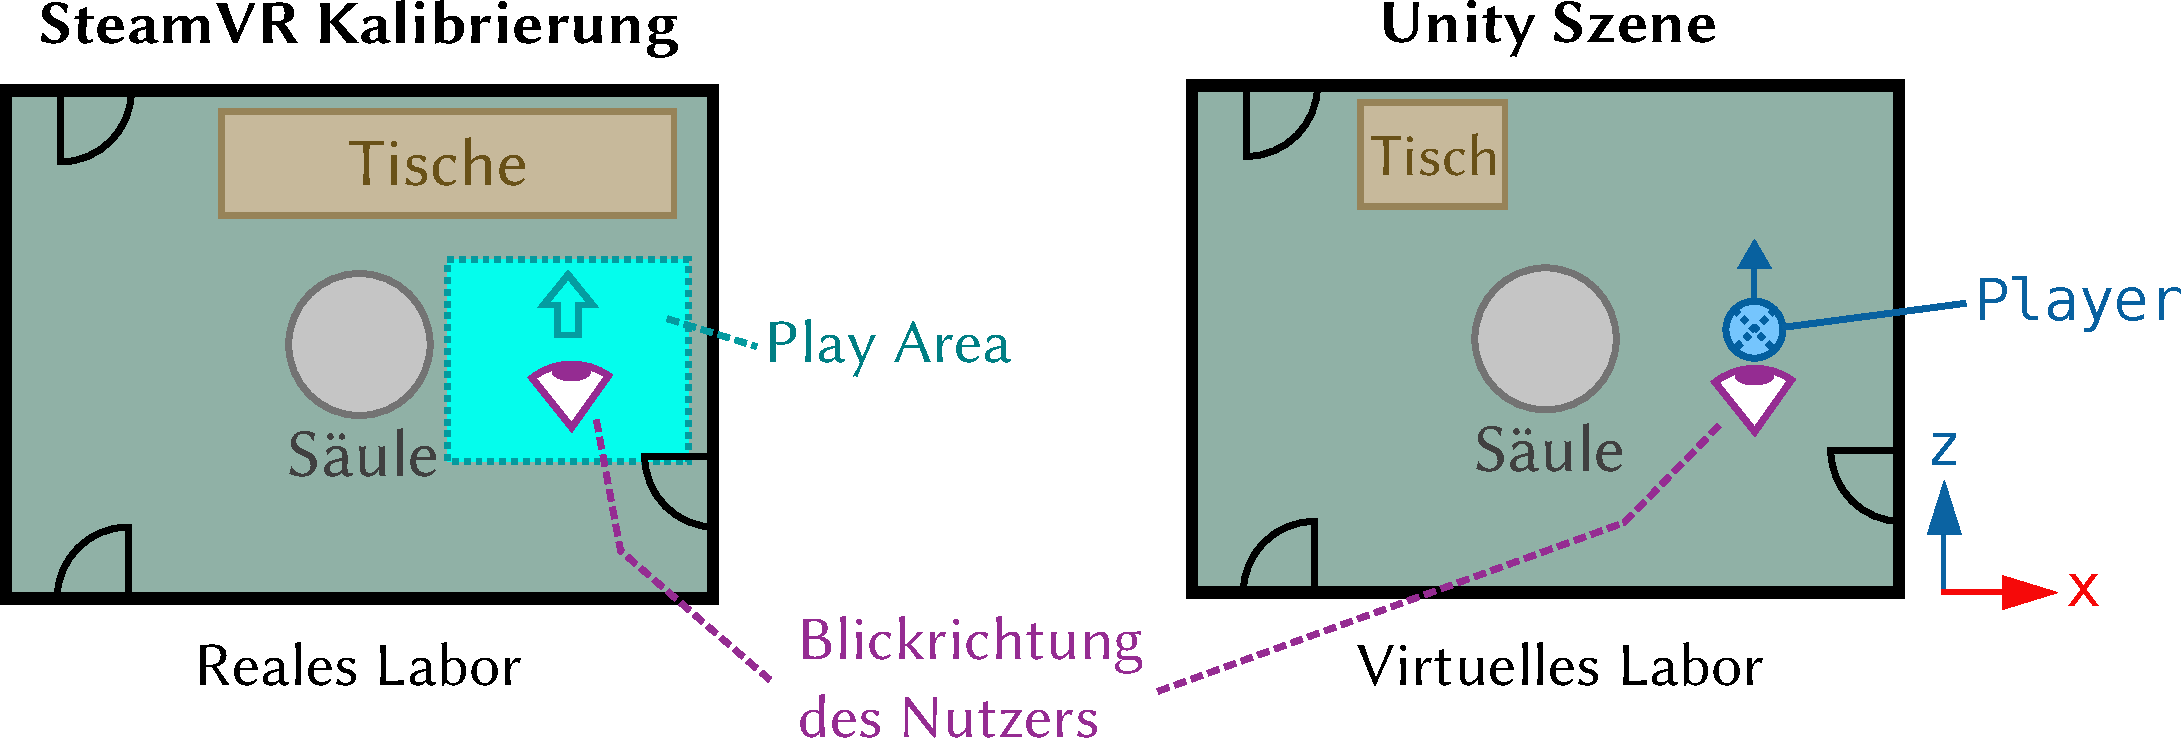
\includegraphics[width=\textwidth]{figures/environment_setup_correct}
    \caption{Die Play Area hat die gleiche Ausrichtung wie das \lstinline{Player}-Objekt in der Grundrotation (entlang z-Achse). %
    Die Rotation des Nutzers in der realen und virtuellen Welt stimmt überein.}
    \label{fig:ve_setup_correct}
\end{figure}

\begin{figure}
    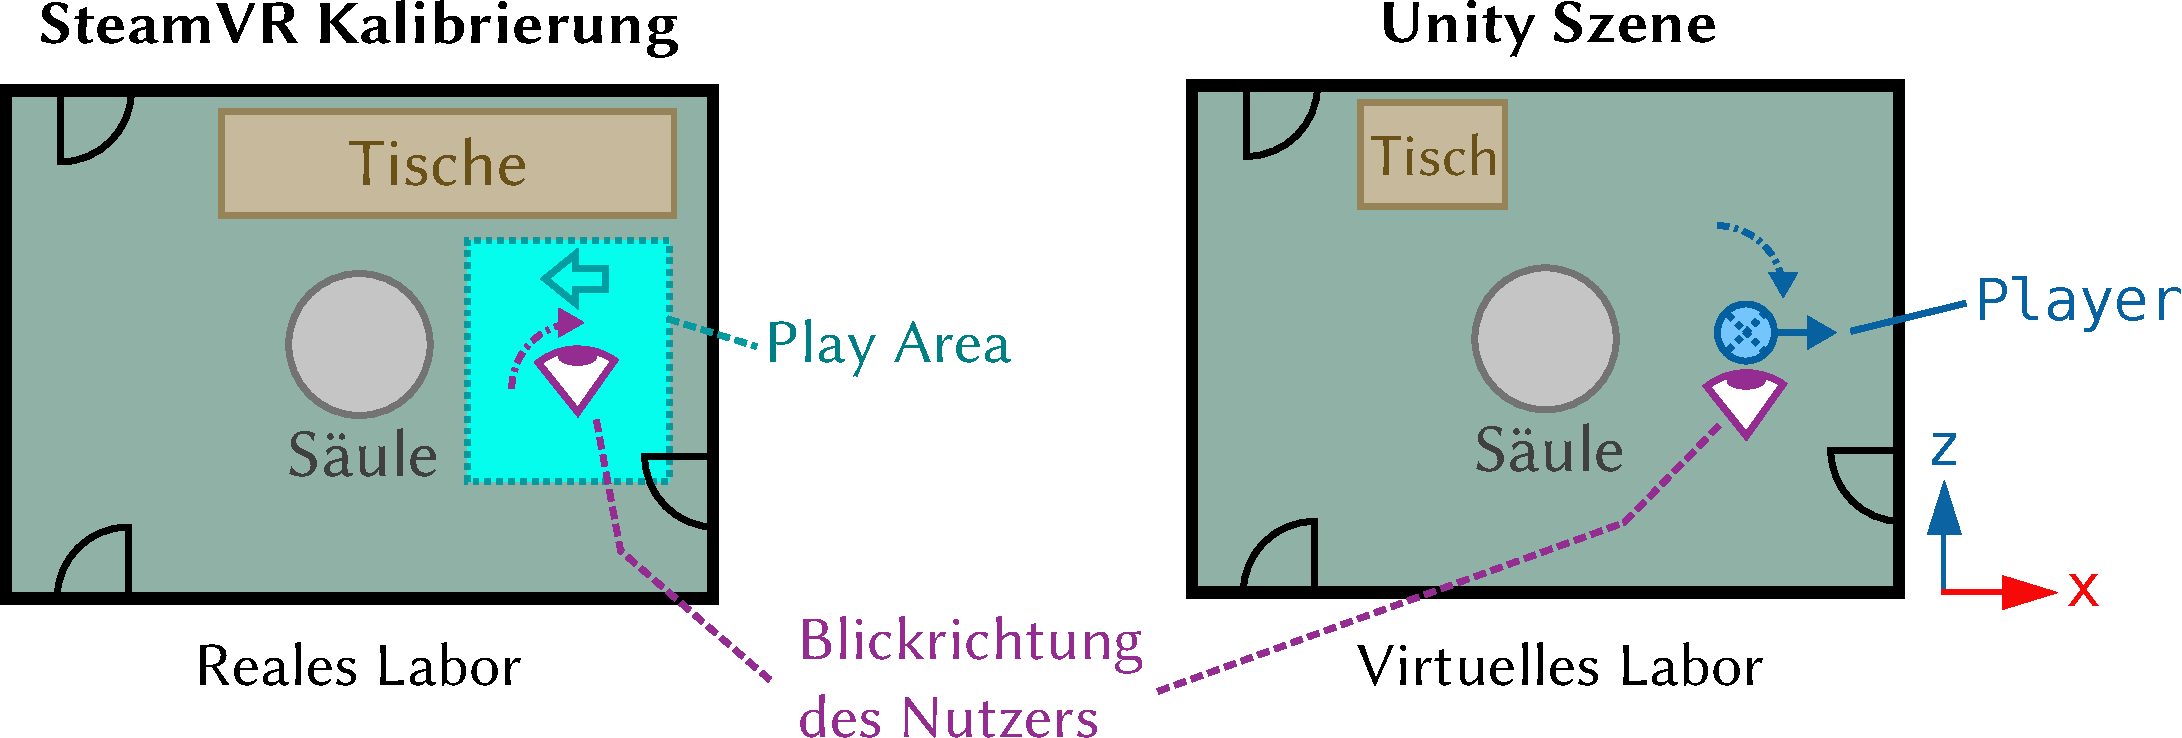
\includegraphics[width=\textwidth]{figures/environment_setup_wrong}
    \caption{Die Play Area hat \emph{nicht} die gleiche Ausrichtung wie das \lstinline{Player}-Objekt in der Grundrotation. %
        Der Nutzer hat einen Rotationsoffset (hier \ang[detect-weight=true]{90}), wodurch für den Nutzer effektiv die Räume unterschiedlich rotiert wirken.}
    \label{fig:ve_setup_wrong}
\end{figure}

\paragraph{Zweiter Schritt:}
Neben der Orientierung des Nutzers muss die Position des virtuellen Raums angepasst werden, wenn dieser die reale Umgebung bestmöglich überlagern soll.
Dies resultiert (wie bei der Rotation) aus der Tatsache, dass die getrackte Position des HMDs im Bezug zur Play Area gemessen wird, welche sich durch den Kalibrierungsvorgang von SteamVR ändern kann.
Um neue Position des virtuellen Raums zu bestimmen wird für den Prototypen wie folgt vorgegangen:

Der Prototyp wird mit seiner Ausgangsposition im Unity Editor ausgeführt.
Die Ecke \enquote{links unten} aus Vogelperspektive des virtuellen Labors befindet sich an der Unity-Welt-Koordinate $(0, 0, 0)$.
Die Controller, welche im HMD durch 3D-Modelle visualisiert sind, werden in den Ecken des virtuellen Raums platziert.
Dabei wird darauf geachtet, dass sie von den Basisstationen weiterhin erkannt werden.
Nun wird im realen Labor die Entfernung von den Controllern zu den entsprechenden Ecken des Raums gemessen, was der Abweichung der virtuellen Welt entspricht.
Die Entfernungen werden gemittelt.
Der resultierende Offset wird dann im Unity Editor verwendet, um das virtuelle Labor zu verschieben.
Dieser Offset ist nun solange gültig, bis die Play Area neu kalibriert wird.
Wie auch schon bei der Rotation ist diese Angleichung erst dann für die Nutzer bemerkbar, wenn sie versuchen physische Objekte wie Wände oder die Säule zu berühren.
Würde die Verschiebung des Raums nicht durchgeführt werden, könnten Nutzer mit den Controllern durch die virtuellen Objekte hindurch greifen oder sie würden auf physische Barrieren stoßen, obwohl die virtuellen Objekte noch weiter entfernt sind.
Nach diesen beiden Schritten kann der virtuelle Raum als Ersatz für die reale Umgebung verwendet werden, die in einer MR-Anwendung ohne vorheriges Modellieren verfügbar wäre.

\section{Das Megamap-GameObject}
\begin{figure}[t]
    \centering
    \imagebox{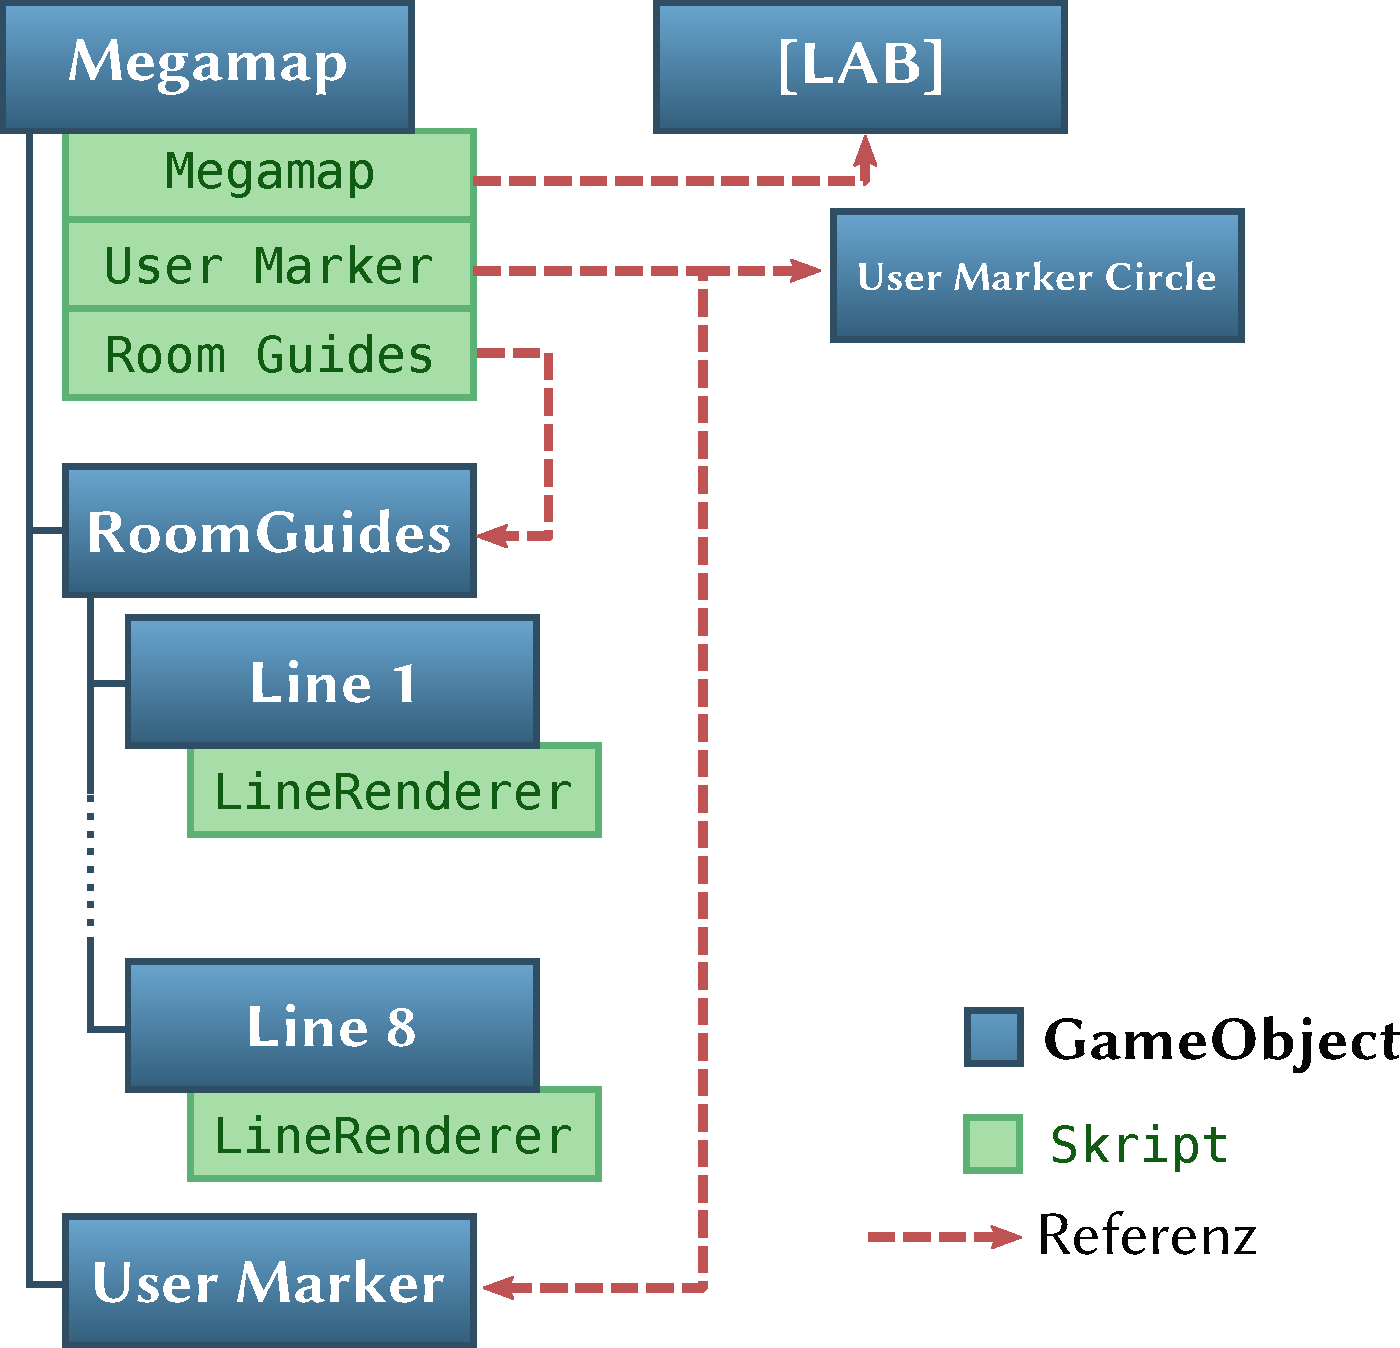
\includegraphics[height=8.5cm]{figures/unity_megamap_object}}
    \caption{Übersicht des Megamap-GameObjects.}
    \label{fig:unity_megamap_object}
\end{figure}

Eine grundlegende Implementierung des in \autoref{chap:concept} vorgestellten Megamap-Konzepts wird im Megamap-GameObject realisiert.
Eine strukturelle Übersicht des Objekts wird in \autoref{fig:unity_megamap_object} gegeben.
Das Objekt setzt sich aus drei Teilen zusammen, die jeweils durch eigene Komponenten repräsentiert werden:

Das Skript \textbf{\lstinline{Megamap}} bietet allgemeine Einstellungsmöglichkeiten zur Darstellung der Megamap.
Es lassen sich z.B. die Skalierung oder die Höhe vom Boden ändern.
Weiterhin bietet das Skript die Methoden \lstinline{Show()} und \lstinline{Hide()}, mit denen die Karte angezeigt bzw. ausgeblendet werden kann.
Falls dabei das Feld \lstinline{useAnimation} auf \lstinline{true} gesetzt ist, wird die Karte beim Anzeigen von einer 1:1 Raumgröße auf die eingestellte Skalierung nach und nach herunterskaliert (beim Ausblenden analog ein Hochskalieren).
Die Megamap wird standardmäßig Nutzer-zentriert platziert.
Das bedeutet, dass der Nutzer sowohl in der realen Welt als auch auf der Karte die gleiche Position einnimmt.
Hierfür wird die virtuelle Umgebung referenziert und der Abstand vom HMD zum Ursprung des Labor-Modells ermittelt.
Dieser Abstand wird dann wie die Megamap skaliert und die Karte wird um den skalierten Abstand verschoben.
Sowohl die Animation als auch die Zentrierung auf den Nutzer sollen es ihm erleichtern, seine eigene Position auf der Karte zu finden.
Außerdem soll hierdurch der Bezug vom Laborraum auf der Karte zum umgebenden Laborraum hervorgehoben werden.

Das \lstinline|Megamap|-Skript dient lediglich als Schnittstelle zur Manipulation der Karte.
Das eigentliche 3D-Modell, welches als Karte verwendet wird, ist von diesem Skript unabhängig und wird erst zur Laufzeit durch andere Skripte als aktive Karte gesetzt.
Hierfür bietet das \lstinline|Megamap|-Skript die Methode \lstinline|SetMap(...)| an, welche als Parameter unter anderem eine Referenz auf ein \lstinline|IndoorMap|-Skript erwartet.
Dank dieser Trennung von Schnittstelle und Modell können zur Laufzeit unterschiedliche Indoor-Karten gewechselt werden, was für die Nutzerstudie in \autoref{chap:evaluation} Voraussetzung ist.
Die Details zum \lstinline|IndoorMap|-Skript werden in \autoref{sec:indoor_maps} ausgeführt.

\begin{figure}
    \centering
    \begin{minipage}[t]{.485\textwidth}
        \centering
        \vspace{0pt}
        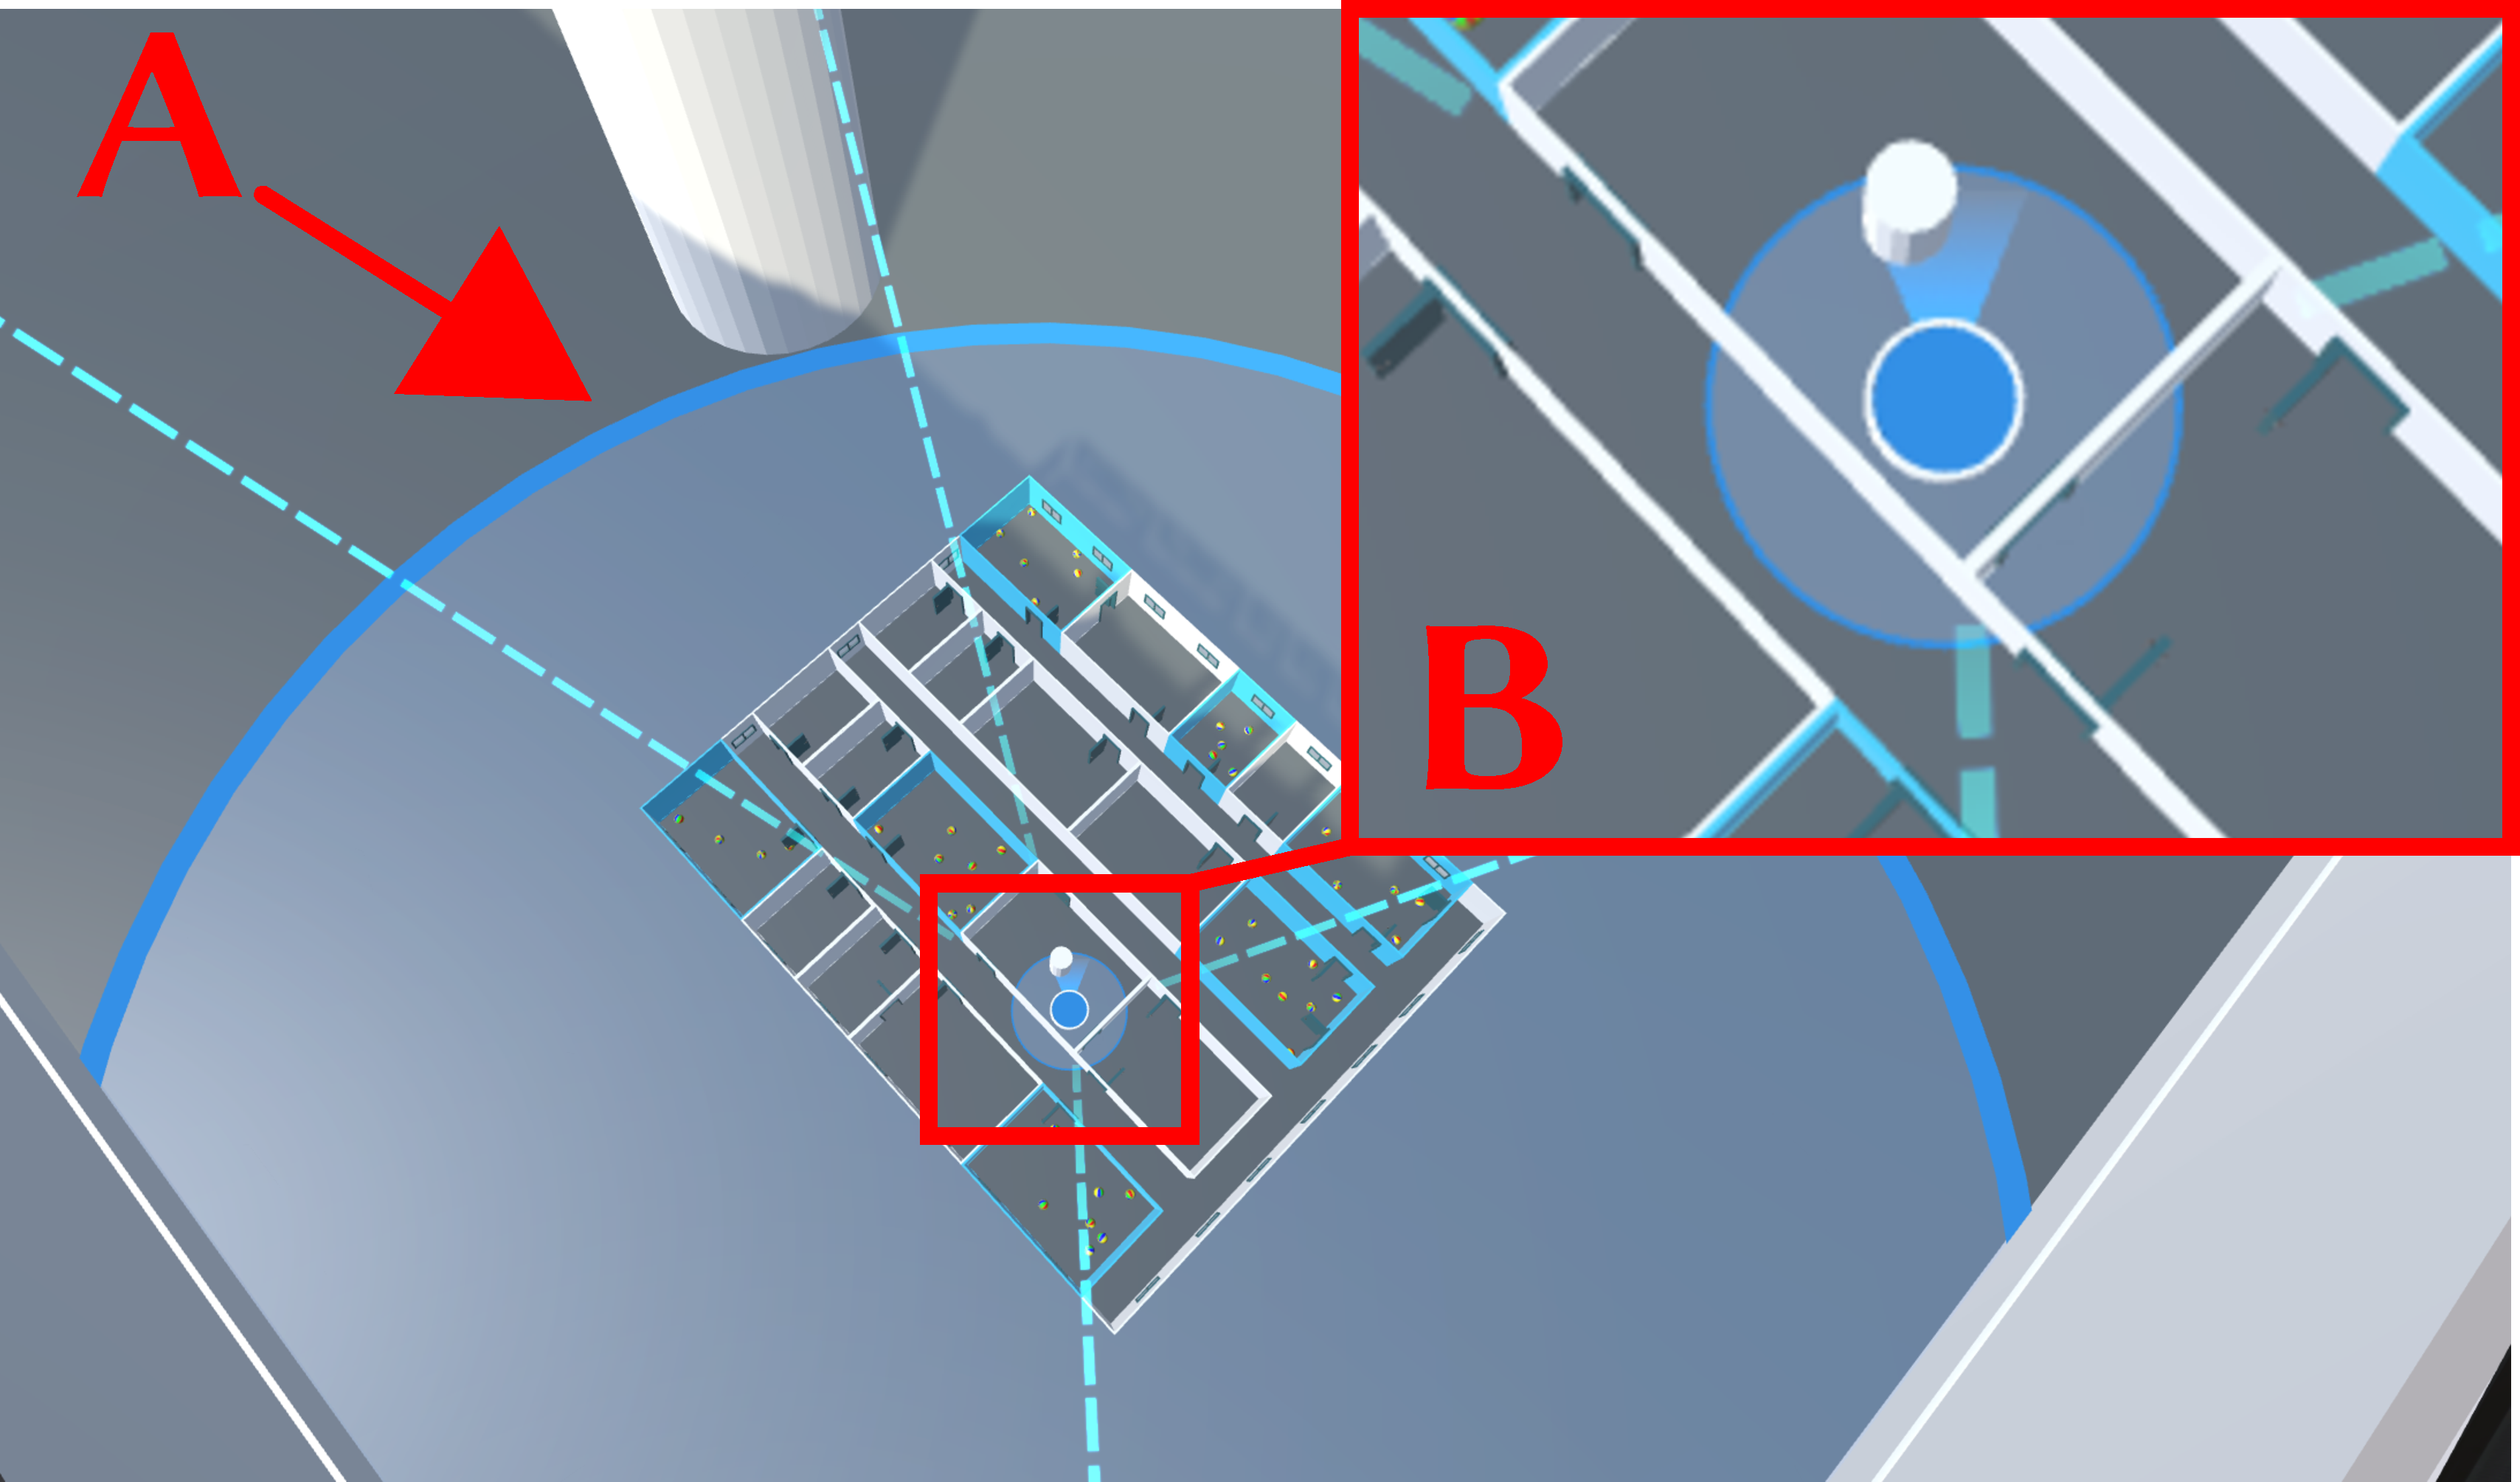
\includegraphics[width=\linewidth]{figures/megamap_user_marker.pdf}
        \captionof{figure}{Der User Marker zeigt die Position des Nutzers auf der Megamap an. %
            \textcolor{red}{A:} Marker in Umgebung. %
            \textcolor{red}{B:} Marker auf Karte.%
        }
        \label{fig:user_marker}
        \vfill
    \end{minipage}
    \hfill
    \begin{minipage}[t]{.485\textwidth}
        \centering
        \vspace{0pt}
        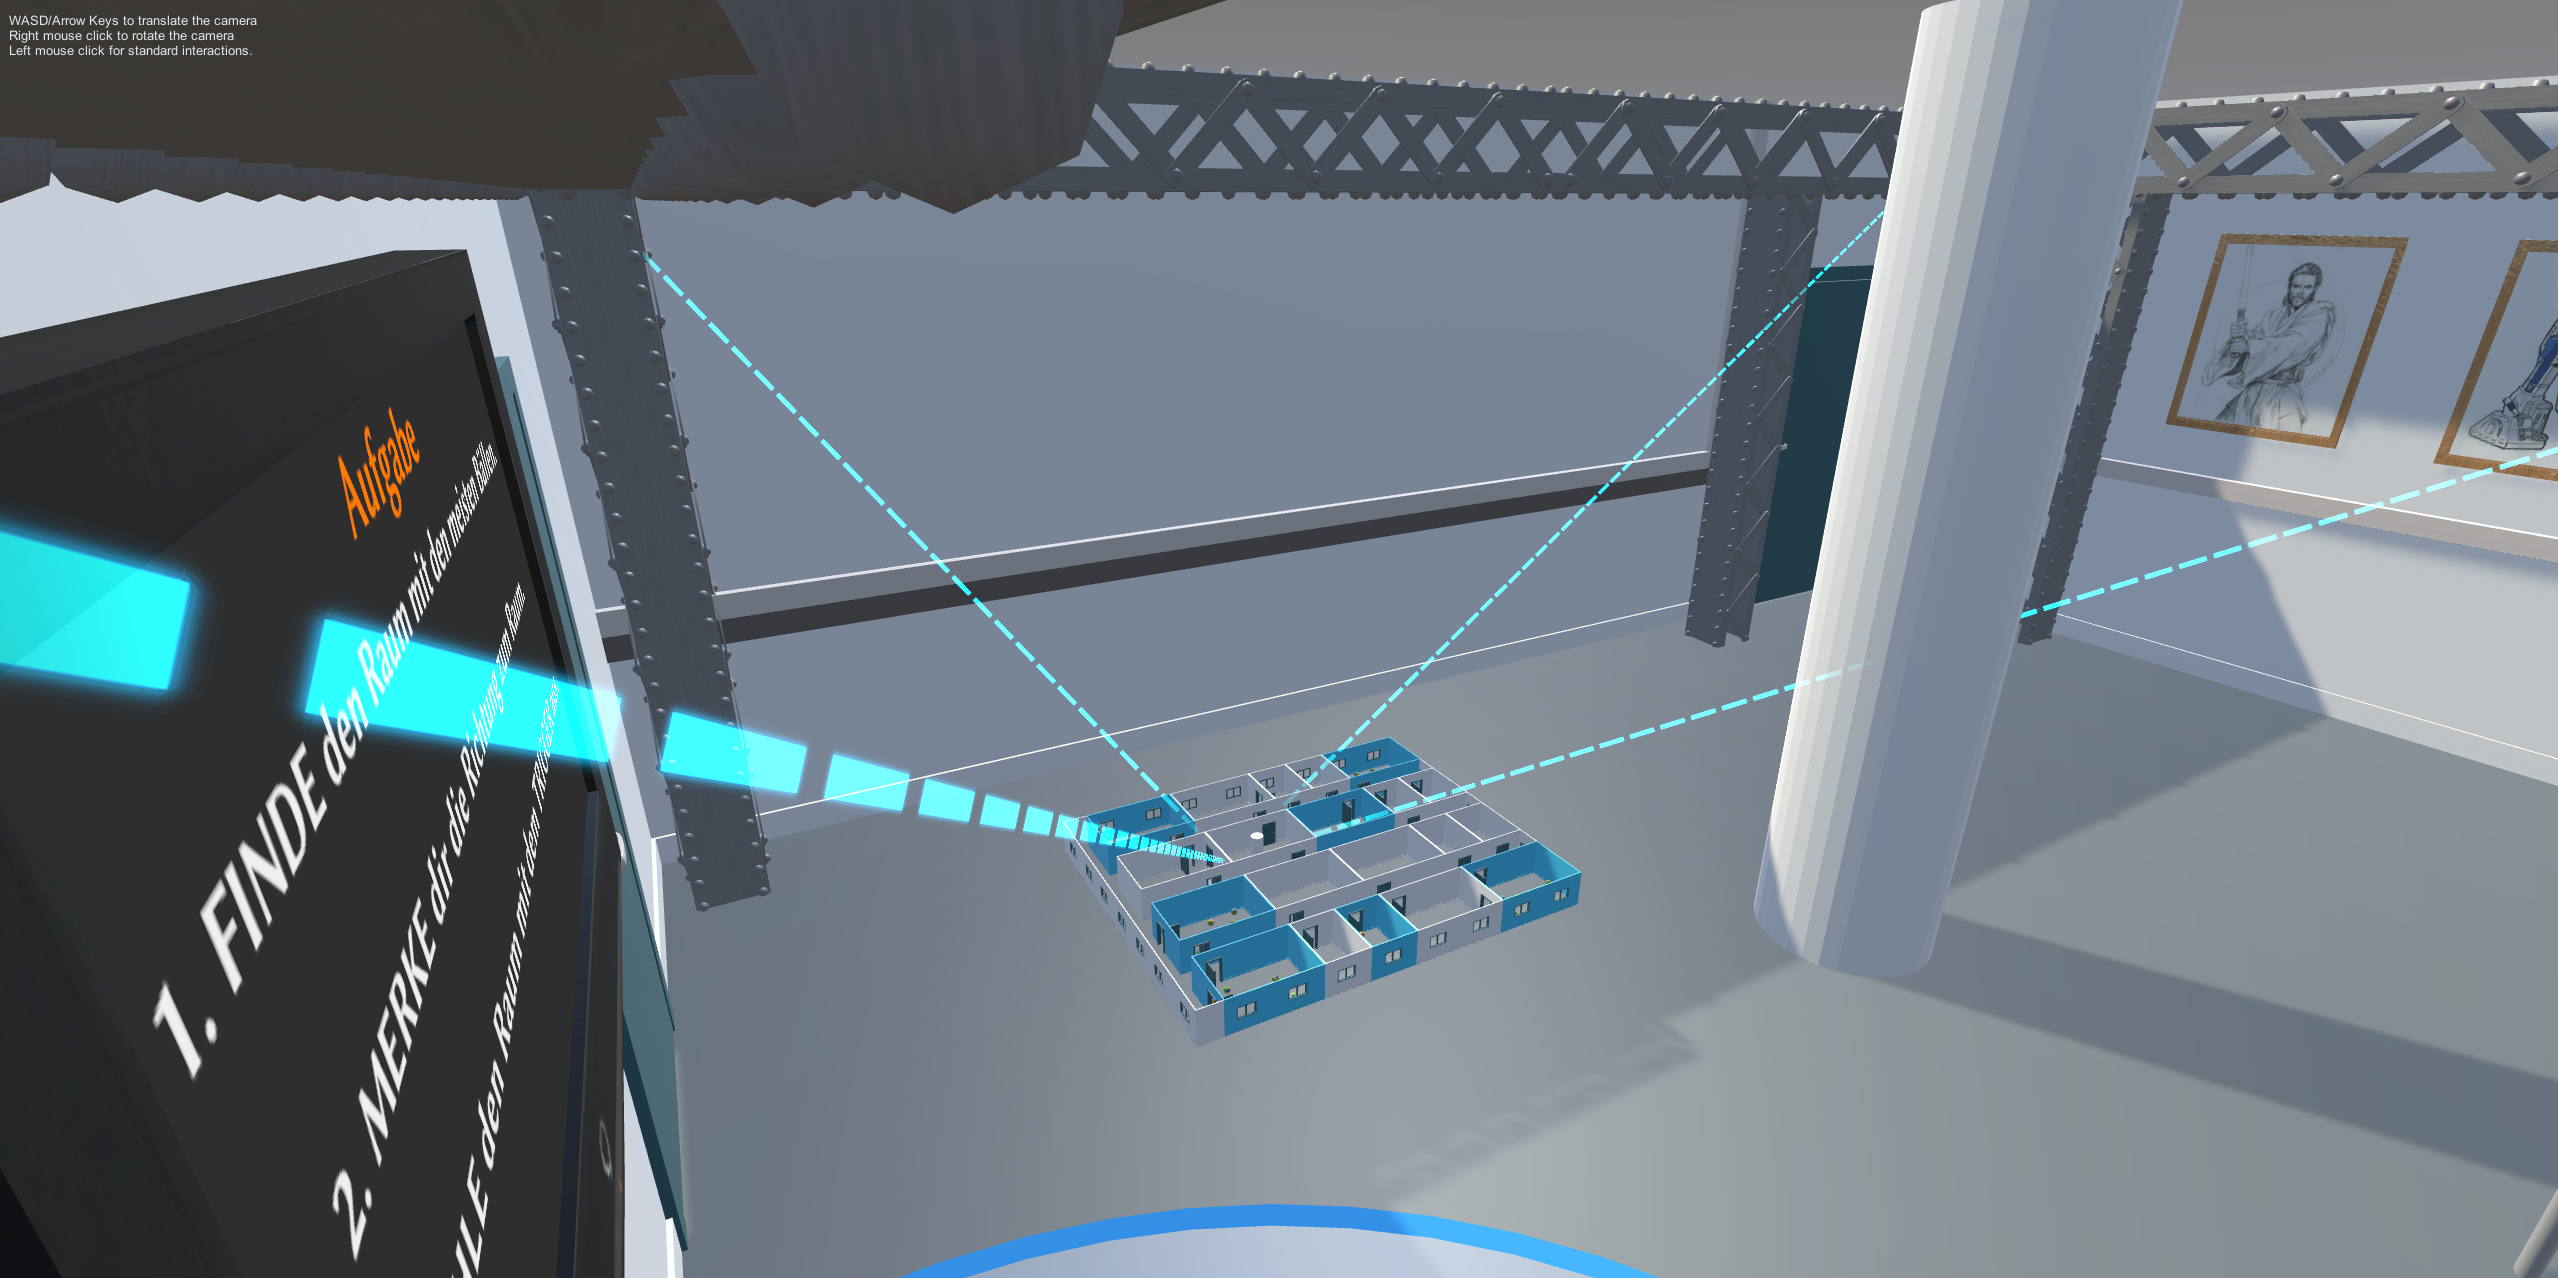
\includegraphics[width=\linewidth, height=4.2cm]{figures/megamap_room_guides}
        \captionof{figure}{Die Room Guides verbinden die Ecken des umgebenden Raums mit dem entsprechenden Raum auf der Megamap.}
        \label{fig:room_guides}
    \end{minipage}
\end{figure}

Der zweite Teil des Megamap-Objekts, das \textbf{\lstinline|User Marker|} Skript, dient ebenfalls der Orientierung für den Nutzer.
Analog zu Kartenanwendungen wie Google Maps befindet sich ein Marker auf der Megamap, welcher die aktuelle Position des Nutzers anzeigt.
Da es sich bei der Megamap um eine dreidimensionale Karte handelt wird hier ein Zylinder in Form ähnlich eines Pucks benutzt (siehe \autoref{fig:user_marker}).
Mittels eines transparenten Kreissegments wird außerdem die aktuelle Rotation des Nutzers verdeutlicht.
Um den Bezug vom Marker auf der Karte zur Umgebung zu verstärken ist auch in dieser ein Kreis platziert, welcher auf dem Nutzer zentriert ist.

Der dritte Teil des Megamap-Objekts ist das \textbf{\lstinline|Room Guides|} Skript.
Durch dieses werden Linien von den Ecken des umgebenden Laborraums zum Laborraum auf der Karte gezogen (siehe \autoref{fig:room_guides}).
Die Linien heben den Raum hervor, in dem sich der Nutzer befindet und stellen somit einen Bezug zur Umgebung her.
Implementiert sind diese Führungslinien als acht \lstinline|GameObject|s mit jeweils einer \lstinline|LineRenderer|-Komponente, die zusammen mit der Megamap ein- bzw. ausgeblendet werden.
Für die Startpunkte der Linien (die Ecken des umgebenden Raums) wird über die \lstinline|Renderer|-Komponente des Labor-Modells auf dessen \emph{Bounding Box} zugegriffen.
Die Eckpunkte der Bounding Box sind die Startpunkte der Linien.
Die Endpunkte der Linien werden berechnet, indem die Startpunkte mit der Transformationsmatrix der Megamap multipliziert werden.
So entsteht der Effekt, dass die Linien zu den Eckpunkten des Labors auf der Karte hinführen.
Standardmäßig werden über das Feld \lstinline|showUpperOnly| nur die oberen vier Linien angezeigt, da die unteren Führungslinien vom Rest der Megamap verdeckt werden würden.

\section{Erstellung der Indoor-Karten}
\label{sec:indoor_maps}
Wie bereits erwähnt ist das eigentliche 3D-Modell, welches das Layout des Gebäudes repräsentiert, vom \lstinline|Megamap|-Skript getrennt.
Für den in dieser Arbeit entwickelten Prototypen werden vorab erstellte 3D-Modelle eingesetzt, die in Blender mit dem Archimesh-Werkzeug modelliert wurden.
Ansätze zur automatisierten Generierung von Gebäudemodellen werden in \autoref{sec:building_data_automation} untersucht.

Die erstellten Karten sind 3D-Modelle, bei denen die einzelnen Räume als separate GameObjects in Unity verfügbar sind.
\autoref{fig:room_hierarchy} zeigt schematisch, wie die Objekthierarchie für die Indoor-Karten in Unity aufgebaut ist.

Für die Nutzerstudie aus \autoref{chap:evaluation} ist es notwendig, dass Nutzer mit Räumen interagieren können.
Es wird eine Suchaufgabe implementiert, bei der die Nutzer den Raum finden müssen, der die meisten Bälle enthält.
Die Nutzer können mit den Vive-Controllern Räume anvisieren und durch Betätigung des Triggers auswählen.
Handelt es sich um den gesuchten Raum, wird die Karte ausgeblendet.
Ansonsten wird der Raum als \enquote{falscher Raum} hervorgehoben.

\begin{figure}[tbh]
    \centering
    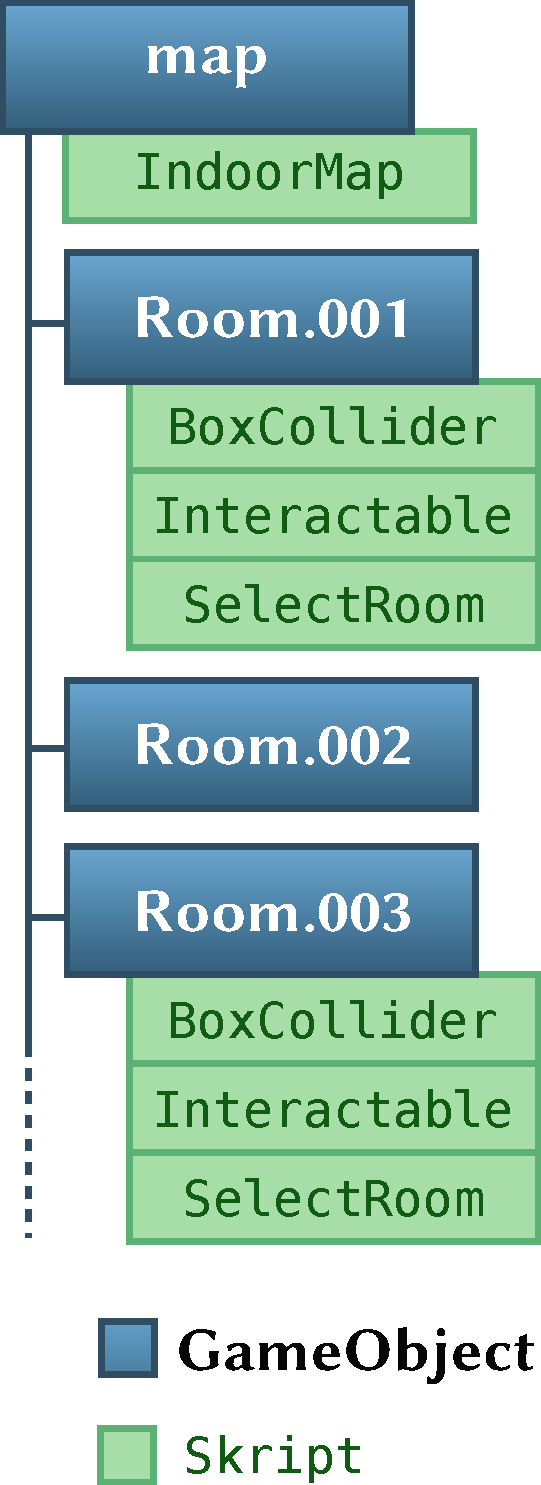
\includegraphics[height=9cm]{figures/unity_indoor_map}
    \caption{Objekthierarchie des IndoorMap-Objekts,}
    \label{fig:room_hierarchy}
\end{figure}

Diese Interaktionsmöglichkeit wird durch das \lstinline|SelectRoom|-Skript umgesetzt.
Das Skript verwendet die SteamVR-Komponente \lstinline|Interactable|, wodurch Räume auf An\-nä\-he\-rungs- und Interaktionsevents der Vive-Controller reagieren können.
Im Skript werden dazu spezielle SteamVR-Methoden implementiert.
Die Methode \lstinline|OnHandHoverBegin(...)| wird ausgelöst, sobald die \lstinline|HoverTransform| des Vive-Controllers den Collider des Raums berührt.
In der Methode wird der Raum gelb hervorgehoben, wenn er zuvor nicht angeklickt wurde.
Wenn er zuvor bereits angeklickt wurde (und nicht der gesuchte Raum ist) wird der Raum stattdessen rot eingefärbt.

Die Methode \lstinline|OnHandHoverEnd(...)| setzt die Farbe des Raums in den Normalzustand zurück, wenn der Vive-Controller den Collider des Raums verlässt.
Somit ist die farbliche Änderung nur sichtbar, solange der Raum mit dem Controller anvisiert wird.

Die \lstinline|HandHoverUpdate(...)|-Methode wird in jedem Update-Iteration von Unity ausgeführt, solange der Vive-Controller den Collider des Raums überlappt.
In der Methode wird überprüft, ob aktuell der Trigger des Controllers betätigt wird.
Sobald der Trigger vom Nutzer gedrückt wird, wird ein Event ausgelöst, was die Auswahl eines Raums signalisiert.
Handelt es sich dabei um den gesuchten Zielraum, wird das Event \lstinline|OnTargetRoomSelected| ausgelöst.
Dieses wird an anderer Stelle benutzt, um die Karte bei Auswahl des Zielraums auszublenden.
Wenn der falsche Raum gewählt wird, wird stattdessen das Event \lstinline|OnWrongRoomSelected| aktiviert.
Dieses wird genutzt, um die Auswahl von falschen Räumen zu zählen und in \autoref{chap:evaluation} auszuwerten. 

Um den Zugriff auf die Räume zu vereinfachen verfügt das IndoorMap-Objekt über das gleichnamige Skript \lstinline|IndoorMap|.
Dieses bietet C\#-Eigenschaften (\emph{Properties}) an, um die Liste aller Räume bzw. die Liste aller \emph{auswählbarer} Räume zu erhalten (\lstinline|Rooms| bzw. \lstinline|SelectableRooms|).

Damit die Megamap das IndoorMap-Objekt als Karte verwendet wird es an die Methode \lstinline|SetMap(...)| des \lstinline|Megamap|-Skripts übergeben.
Hierdurch wird das IndoorMap-Objekt zu einem Kind-Objekt der Megamap.
Die Skalierung und Translation der Megamap werden automatisch für das Kartenmodell übernommen.
Die Karte kann durch weitere Aufrufe von \lstinline|SetMap(...)| ausgetauscht werden.

\section{Interaktion mittels virtuellem Laserpointer}
Mit den \lstinline|SelectRoom|- und \lstinline|Interactable|-Skripten können Nutzer die Räume auf der Karte mit dem Vive-Controller auswählen.
Allerdings müssten sie sich (ohne weitere Maßnahmen) zu den einzelnen Räumen hinbewegen, um diese mit dem Vive-Controllern zu berühren und auszuwählen.
In informellen Vortests des Prototypen zeigte sich, dass die Bewegung zu den Räumen umständlich ist, wenn lediglich ein einzelner Raum gefunden werden soll.
Die Play Area der Vive schränkt die Bewegung der Nutzer zusätzlich ein, da außerhalb der Play Area mit Hindernissen gerechnet werden muss und das Tracking durch die Basisstationen ungenauer wird.

Für den aktuellsten Prototyp wurde daher eine Methode zur entfernten Auswahl von Räumen entwickelt.
Über einen virtuellen \enquote{Laser Pointer} können Nutzer mit den Vive-Controllern auf Räume zeigen und diese mit dem Trigger auswählen.
Der Screenshot in \autoref{fig:laserpointer_screenshot} zeigt ein Beispiel.
Das Skript \lstinline|LaserPointer| setzt dies um, indem es einen \lstinline|LineRenderer| aktiviert, welcher einen Lasterstrahl darstellt.
Der Strahl verläuft vom Controller geradeaus in die Szene.
In der Methode \lstinline|Update()| wird dann durch \lstinline|Physics.RaycastAll(...)| ein Schnitttest zwischen dem Strahl und Collidern in der Szene durchgeführt.
Falls ein Collider vom Strahl getroffen wird und der Collider zu einem der Räume gehört, wird der Schnittpunkt als Endpunkt des Laserstrahls gesetzt.
So entsteht der Effekt, dass der Laserstrahl nicht durch die Räume hindurchgeht.
\begin{figure}[htb]
    \centering
    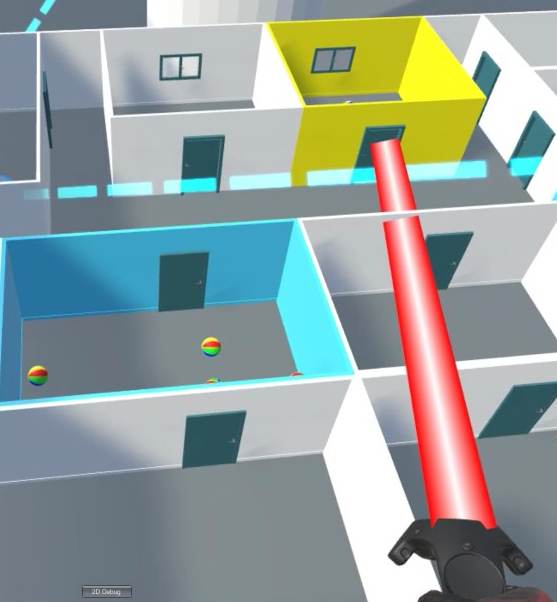
\includegraphics[height=6cm]{figures/screenshots/laserpointer}
    \caption{Mit dem Laserpointer wird ein Raum anvisiert.}
    \label{fig:laserpointer_screenshot}    
\end{figure}

Wie im vorigen Abschnitt beschrieben findet die Interaktion zwischen Vive-Controller und einem Raum statt, wenn der Controller den Raum überlappt.
Da jedoch beim Laserpointer der Controller vom Raum entfernt ist, muss hier eine Modifikation vorgenommen werden.
Intern nutzt das SteamVR-\lstinline|Hand|-Skript (welches den Controller repräsentiert und trackt) die Felder \lstinline|HoverSphereTransform| und \lstinline|HoverSphereRadius|.
Beide Felder definieren eine unsichtbare Kugel mit einem gegebenen Radius.
Standardmäßig folgt diese Kugel der Position des Controllers.
Sobald die Kugel mit einem \lstinline|Interactable|-Objekt überlappt, werden die entsprechenden SteamVR-Events ausgelöst.
Für den Laserpointer wird diese Kugel verschoben, wenn der Raycast einen Schnittpunkt mit einem auswählbaren Raum ergibt.
Die Position der Kugel wird auf den Schnittpunkt geändert, wodurch sie sich effektiv am Ende des Laserstrahls befindet.
Damit werden die SteamVR-Events für den entsprechenden Raum am Ende des Strahls ausgelöst.
\autoref{fig:laserpointer_sketch} verdeutlicht diesen Vorgang.
Wenn der Raycast keinen Schnittpunkt mit einem auswählbaren Raum ergibt, wird die Kugel wieder auf die Controller-Position zurückgesetzt.
\begin{figure}[hbt]
    \centering
    \imagebox{%
    \begin{subfigure}{0.45\linewidth}
        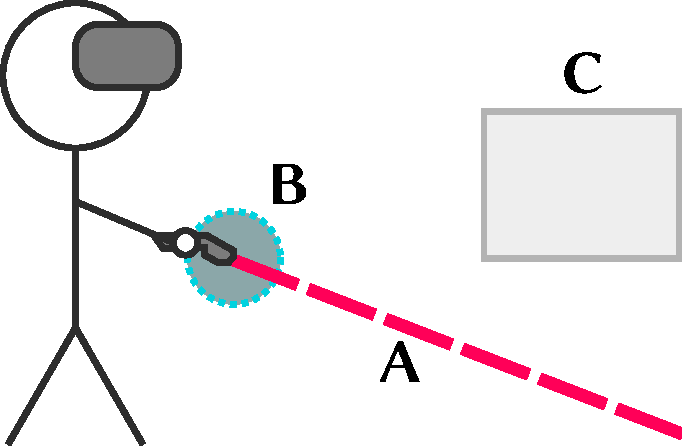
\includegraphics[width=\linewidth]{figures/laserpointer_sketch_no_hit}
        \caption{}
        \label{sfig:laserpointer_sketch_no_hit}
    \end{subfigure}
    \hfill
    \begin{subfigure}{0.45\linewidth}
        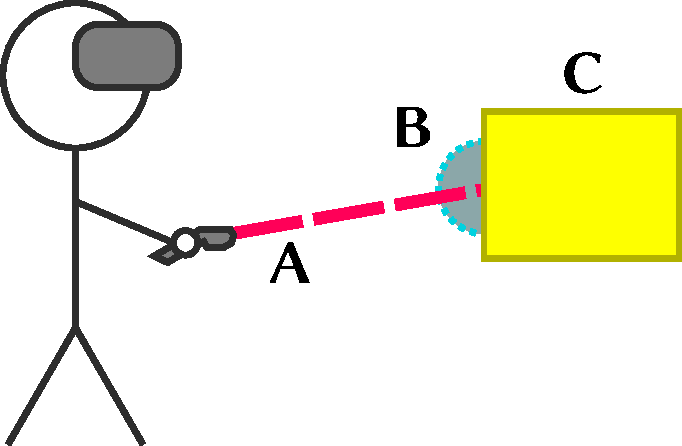
\includegraphics[width=\linewidth]{figures/laserpointer_sketch_hit}
        \caption{}
        \label{sfig:laserpointer_sketch_hit}
    \end{subfigure}
    }
    \caption{Funktionsweise des Laserpointers. %
        Die \lstinline|HoverSphere| wird verschoben, sodass der Raum auf den Vive-Controller reagiert. %
        \textbf{A:} Laserpointer. \textbf{B:} SteamVR-\lstinline|HoverSphere|. \textbf{C:} Auswählbarer Raum.}
    \label{fig:laserpointer_sketch}
\end{figure}

%
\cleardoublepage


\printbibliography[heading=bibintoc, nottype=online]
\printbibliography[heading=bibintoc, title={Online Referenzen}, type=online]

\end{document}
